\documentclass[dvipsnames,12pt]{book}
\usepackage{tikz}
\usepackage[hypcap=true]{caption}

\graphicspath{{Images/}}

%Hey, if you're using this preamble it means that it was probably written by Stefano Graziosi (me). If you see something that doesn't make sense, feel free to email me at stefano.graziosi@studbocconi.it
%p.s. in case it's not already evident from the preamble, I'm not a professional LaTeX user, so I'm sure there are better ways to do things. I'm just trying to make it work.

%------------------------------------------------------------------------------
%           LAST UPDATE: 30-01-2025
%------------------------------------------------------------------------------

%I don't own copyright on anything, I just literally copied and pasted together a bunch of stuff.

%Credit goes to the original authors.

%------------------------------------------------------------------------------
%           Packages
%------------------------------------------------------------------------------

\usepackage{fancyhdr}
\usepackage[dvipsnames]{xcolor}
\usepackage[many]{tcolorbox}
\usepackage[all]{xy}
\usepackage{tcolorbox}
\usepackage{graphicx}
\usepackage{hyperref}
\usepackage{xcolor}    
\usepackage{wrapfig}
\usepackage{amsmath, amssymb, amsthm}
\usepackage{titlesec}
\usepackage{halloweenmath}
\usepackage{enumitem}
\usepackage{listings}

\usepackage[T1]{fontenc}                            % Font Styling
\usepackage{lmodern,mathrsfs}


\usepackage{mathtools,amsthm,amssymb,amsfonts,bm}   % Math Presets
\usepackage{thmtools,amsmath}
\usepackage{array,tabularx,booktabs}                % Table Presets
\usepackage{graphicx,wrapfig,float,caption}         % Figure Presets
\usepackage{setspace,multicol}                      % Text Presets
\usepackage{tikz,physics}                           % Physics Presets

\usepackage{titlepic}
\usepackage{pdfpages}

%------------------------------------------------------------------------------
%           Geometry
%------------------------------------------------------------------------------

\usepackage[a4paper,margin=1in]{geometry}
%\usepackage[margin=1in]{geometry}

\renewcommand{\chaptername}{Lecture}
%\renewcommand\thesection{P~\arabic{section}}

%------------------------------------------------------------------------------
%           Colours
%------------------------------------------------------------------------------

\definecolor{sgblue}{rgb}{0, 169, 211}
\definecolor{sggreen}{rgb}{0, 164, 0}
\definecolor{sgpurple}{rgb}{99, 0, 165}
\definecolor{sgyellow}{rgb}{255, 211, 0}
\definecolor{sgorange}{rgb}{255, 127, 20}

\definecolor{sbblue}{rgb}{219, 248, 254}
\definecolor{sbgreen}{rgb}{223, 255, 218}
\definecolor{sbpurple}{rgb}{241, 220, 255}

\definecolor{codegreen}{rgb}{0,0.6,0}
\definecolor{codegray}{rgb}{0.5,0.5,0.5}
\definecolor{codepurple}{rgb}{0.58,0,0.82}
\definecolor{backcolour}{rgb}{0.95,0.95,0.92}

%------------------------------------------------------------------------------
%           Environments
%------------------------------------------------------------------------------

%Standard \latex box

\newtcolorbox{mybox}[3][]
{
  colframe = #2!25,
  colback  = #2!10,
  coltitle = #2!20!black,  
  title    = {#3},
  #1,
}

%Standard "Problem" environment

\newtheorem{problem}{Problem}

%Personalised "Solution" environment

\newenvironment{solution}[1][\it{\textcolor{MidnightBlue}{Solution}}]{\textbf{#1. } }{\textcolor{MidnightBlue}{$\square$}}


% ----------------------------------------------------------------------
%           Special Environments 
% ----------------------------------------------------------------------

\newlength{\spacelength}
\settowidth{\spacelength}{\normalfont\ }
\declaretheoremstyle[
    headfont={\bfseries\sffamily\footnotesize},
    notefont={\normalfont},
    bodyfont={\normalfont},
    headpunct={\relax},%\newline,
    headformat={%
        \makebox[0pt][r]{\NAME\ \NUMBER\hspace{\marginparsep}}\hskip-\spacelength{\normalsize\NOTE}},
]{theorem}

\tcolorboxenvironment{theorem}{
  boxrule=0pt,
  boxsep=0pt,
  colback={White},
  enhanced jigsaw, 
  borderline west={1pt}{0pt}{ForestGreen},
  sharp corners,
  before skip=10pt,
  after skip=10pt,
  left=5pt,
  right=5pt,
  breakable,
}

\declaretheorem[style=theorem]{proposition}

\let\proof\relax
\let\endproof\relax

\declaretheoremstyle[
    headfont={\bfseries\sffamily\footnotesize},
    notefont={\normalfont},
    bodyfont={\normalfont},
    headpunct={\relax},%\newline,
    headformat={%
        \makebox[0pt][r]{\NAME\ \NUMBER\hspace{\marginparsep}}\hskip-\spacelength{\normalsize\NOTE}},
]{theorem}

\tcolorboxenvironment{proposition}{
  boxrule=0pt,
  boxsep=0pt,
  colback={White},
  enhanced jigsaw, 
  borderline west={1pt}{0pt}{Mulberry},
  sharp corners,
  before skip=10pt,
  after skip=10pt,
  left=5pt,
  right=5pt,
  breakable,
}

\declaretheorem[style=theorem]{theorem}

\let\proof\relax
\let\endproof\relax

\declaretheoremstyle[
    headfont={\small\scshape},
    notefont={\normalfont},
    bodyfont={\normalfont},
    headpunct={\relax},
    headformat={%
        \makebox[0pt][r]{\NAME\hspace{\marginparsep}}\hskip-\spacelength{\NOTE}},
]{proof}

\tcolorboxenvironment{proof}{
  boxrule=0pt,
  boxsep=0pt,
  blanker,
  borderline west={1pt}{0pt}{black},
  before skip=10pt,
  after skip=10pt,
  left=5pt,
  right=5pt,
  breakable,
}

\declaretheoremstyle[
    headfont={\footnotesize\itshape},
    notefont={\normalfont},
    bodyfont={\normalfont},
    headpunct={\relax},
    headformat={%
        \makebox[0pt][r]{\NAME\hspace{\marginparsep}}\hskip-\spacelength{\NOTE}},
]{claim}

\declaretheorem[
    style=proof,
    qed=\qedsymbol]{proof}

\declaretheorem[style=claim]{Intuition}

\theoremstyle{theorem}
\newtheorem{ques}{Question}

\theoremstyle{theorem}
\newtheorem{definition}{Definition}
\tcolorboxenvironment{definition}{
  boxrule=0pt,
  boxsep=0pt,
  colback={White},
  enhanced jigsaw, 
  borderline west={1pt}{0pt}{Cerulean},
  sharp corners,
  before skip=10pt,
  after skip=10pt,
  left=5pt,
  right=5pt,
  breakable,
}

\theoremstyle{theorem}
\newtheorem{lemma}{Lemma}
\tcolorboxenvironment{lemma}{
  boxrule=0pt,
  boxsep=0pt,
  blanker,
  borderline west={1pt}{0pt}{Rhodamine},
  before skip=10pt,
  after skip=10pt,
  sharp corners,
  left=5pt,
  right=5pt,
  breakable,
}

\theoremstyle{theorem}
\newtheorem{remark}{Remark}
\tcolorboxenvironment{remark}{
  boxrule=0pt,
  boxsep=0pt,
  colback={White},
  enhanced jigsaw, 
  borderline west={1pt}{0pt}{BurntOrange},
  before skip=10pt,
  after skip=10pt,
  sharp corners,
  left=5pt,
  right=5pt,
  breakable,
}

\theoremstyle{theorem}
\newtheorem{corollary}{Corollary}
\tcolorboxenvironment{corollary}{
  boxrule=0pt,
  boxsep=0pt,
%  colback={White!100!WildStrawberry},
  enhanced jigsaw,
  borderline west={1pt}{0pt}{WildStrawberry},
  before skip=10pt,
  after skip=10pt,
  sharp corners,
  left=5pt,
  right=5pt,
  breakable,
}

\theoremstyle{theorem}
\newtheorem{example}{Example}
\tcolorboxenvironment{example}{
  boxrule=0pt,
  boxsep=0pt,
  blanker,
  borderline west={1pt}{0pt}{Dandelion},
  before skip=10pt,
  after skip=10pt,
  sharp corners,
  left=5pt,
  right=5pt,
  breakable,
}


\theoremstyle{claim}
\newtheorem{intu}{Intuition}

\theoremstyle{claim}
\newtheorem{solu}{Solution}

%------------------------------------------------------------------------------
%           Code Listing Environment
%------------------------------------------------------------------------------

\lstdefinestyle{mystyle}{
    backgroundcolor=\color{backcolour},   
    commentstyle=\color{codegreen},
    keywordstyle=\color{magenta},
    numberstyle=\tiny\color{codegray},
    stringstyle=\color{codepurple},
    basicstyle=\ttfamily\footnotesize,
    breakatwhitespace=false,         
    breaklines=true,                 
    captionpos=b,                    
    keepspaces=true,                 
    numbers=left,                    
    numbersep=5pt,                  
    showspaces=false,                
    showstringspaces=false,
    showtabs=false,                  
    tabsize=2
}

\lstset{style=mystyle}

\setlist[itemize]{label=\textbullet}

\titlepic{
    \makebox[0pt][c]{\hspace*{0.135cm}%
    
\includegraphics[width=\paperwidth]{20888 Logo.png}
    }
}
\title{20888 Foundations of Social Sciences - Module 2A \\[0.2cm] {\Large \textit{Institutions, Government and Society}} \\[1cm] \textbf{Lecture Notes}}
\author{Stefano Graziosi, Università Bocconi \\
        Federico Mellace, Università Bocconi}
\date{\today}

\begin{document}

\maketitle

\tableofcontents

\part{History of Economic Thought}

    \chapter[Exchange and Political Community]{Aristotle \\[0.6cm] \textit{Exchange and Political Community}}

            \section{Politics - Book I}

        \subsection{Introduction: The Polis and the Oikos}

            One of Aristotle’s key distinctions in Politics Book I is between the \textit{polis} (the city or political community) and the \textit{oikos} (the household or family). For the ancient Greeks, these two spheres represented fundamentally different realms of human activity:
    
                \begin{definition}[oikos]
                    The \textit{oikos} is the sphere of necessity—it deals with survival, daily needs, and household management.
                \end{definition}
    
                \begin{definition}[polis]
                    The \textit{polis} is the sphere of freedom—it aims at enabling people to live the good life, one marked by virtuous activity and flourishing.
                \end{definition}

            \subsubsection{A Central Question}

                \begin{quote}
                    Should the state be managed as an enterprise or not? Should an entrepreneur manage the state as if it were his enterprise?
                \end{quote}

                This question highlights a tension still relevant today: can (or should) the principles of economic management (focused on profit, efficiency, resource allocation) govern the political realm (focused on justice, common good, and the flourishing of citizens)?
                
                Aristotle’s answer—developed throughout his Politics—is that the methods of running a household economy (oikos) and the methods of running a political community (polis) are necessarily different. Politics, for Aristotle, is not merely a larger-scale version of household management.
\newpage
            \subsection{Digression: Hannah Arendt}

                Hannah Arendt (1906–1975) was a 20th-century political theorist whose works often draw on ancient Greek thought. Two of her major works are:
\vspace{-0.05cm}
                    \begin{itemize}
                        \item \textit{The Origins of Totalitarianism} (1951) – An analysis of totalitarian regimes (Nazi Germany, Stalinist Russia), focusing on how they subverted the public realm and destroyed the capacity for genuine political action.
                        \item \textit{The Human Condition} (1958) – An exploration of what it means to be human in the modern age, distinguishing different kinds of human activities (labor, work, and action) and reflecting on the modern eclipse of authentic political life.
                    \end{itemize}

                \subsubsection{Arendt on “Political Economy”}

                    Arendt famously claimed that the term “\textbf{political economy}” is an \textit{oxymoron}. \textbf{Why?} In antiquity, politics and economics were understood to be distinct spheres:
                            \begin{itemize}
                                \item \textbf{Economics} (oikonomia) is the management of the household (oikos), governed by necessity and the administration of resources.
                                \item \textbf{Politics} (the life of the polis) is the realm of public freedom, speech, and action, dedicated to matters of justice and the common good.
                            \end{itemize}

                    For Arendt, and following Aristotle, conflating these two realms—treating the political community as though it should be run by the same principles as a household or enterprise—distorts the essence of politics, which involves deliberation about the just and the unjust, the good and the bad, and the shared life of citizens.
\vspace{-0.25cm}
                \subsubsection{Arendt’s Three Human Activities}

                    In \textit{The Human Condition}, Arendt distinguishes three fundamental human activities:
\vspace{-0.05cm}
                        \begin{enumerate}
                            \item \textbf{Animal laborans} (the laboring animal)
                                \begin{itemize}
                                    \item Concerned with biological life (eating, sleeping, reproducing).
                                    \item Its tasks are repetitive and cyclical, tied to necessity.
                                \end{itemize}
                            \item \textbf{Homo faber} (the maker or builder)
                                \begin{itemize}
                                    \item Concerned with production or fabrication—crafting things that endure beyond their maker’s lifespan (e.g., art, tools, buildings).
                                    \item Gives the world a degree of permanence and durability.
                                \end{itemize}
                            \item \textbf{Zoon politikon} (the political animal)
                                \begin{itemize}
                                    \item Concerned with action (praxis) and speech, particularly in the public realm.
                                    \item Seeks the good life through debate, deliberation, and collective decision-making, embodying the classic Greek notion of full human flourishing.
                                \end{itemize}
                        \end{enumerate}

                    \begin{remark}
                        In ancient Greece, these spheres were more distinctly separated. Today, modern societies often conflate or subordinate the political (the realm of freedom and debate) to the economic (the realm of necessity and consumption)
                    \end{remark}

                \subsection{Succession and Priority}

                    \begin{remark}[Succession]
                        \textit{oikos} \(\rightarrow\) \textit{kòme} \(\rightarrow\) \textit{polis}
                    \end{remark}
            
                    Aristotle observes a developmental sequence in human communities: from the family (\textit{oikos}), to the village (\textit{kòme}), and finally to the city-state (\textit{polis}). However, he also asserts that the polis is by nature prior to the household and the individual (a statement he elaborates on in Politics 1253a).

                    While it might seem that the household comes “first,” Aristotle’s point is that the fully realized form of human association—the polis—logically and ontologically precedes the household in importance: only within a polis can human beings achieve the higher ends of justice and virtue.
            

        \section{Zoon Politikon}

            In Book I of the Politics, Aristotle famously argues that human beings are political animals (zoon politikon) more so than any other gregarious or social creatures. Unlike bees or ants, which also cooperate, humans have a unique capacity for logos—reasoned speech. This capacity allows us to discuss justice, goodness, advantageous vs. harmful, and other moral distinctions in ways that mere instinctual signalling cannot.

            \begin{quote}
                It is thus clear that man is a political animal (zoon politikon), in a higher degree than bees or other gregarious animals. Nature, according to our theory, makes nothing in vain; and man alone of the animals is furnished with the faculty of language. 
                
                The mere making of sounds serves to indicate pleasure and pain, and is thus a faculty that belongs to animals in general: their nature enables them to attain the point at which they have perceptions of pleasure and pain, and can signify those perceptions to one another.

                But language serves to declare what is advantageous and what is the reverse, and it is the peculiarity of man, in comparison with other animals, that he alone possesses a perception of good and evil, of the just and the unjust, and other similar qualities; and it is association in these things which makes a family (oikos) and a city (polis).

                (Aristotle, Politics 1253a7-18)
            \end{quote}

                \subsubsection{The Role of Language (Logos)}
    
                    \begin{itemize}
                        \item Mere sounds are shared by many animals, indicating pleasure and pain (e.g., growls, screeches).
                        \item Speech (logos) in the human sense involves the articulation of concepts such as justice and injustice, good and evil—a moral dimension unique to human beings.
                    \end{itemize}
    
                    Hence, the capacity for public discourse (deliberation, persuasion, debate) is the foundation of political life. This is why the community that arises from such discourse—the polis—is crucial for human flourishing: we need a public space in which to exercise our capacity to debate justice and the good.

            \subsection{Polis and Oikos}

                \begin{quote}
                    We may now proceed to add that the city (polis) is prior in the order of nature to the family (oikos) and the individual. The reason for this is that the whole is necessarily prior to the part. If the whole body is destroyed, there will not be a foot or a hand, except in that ambiguous sense in which one uses the same word to indicate a different thing, as when one speaks of a ‘hand’ made of stone…

                    (Aristotle, Politics 1253a18-25)
                \end{quote}

                    Aristotle here uses a biological analogy: just as a hand cannot fully exist as a hand if severed from the body, so the household and individual cannot truly exist (in their proper form) apart from the city. This does not deny the importance of families or individuals; rather, it emphasizes that the complete flourishing of each part depends on the whole of which it is a part.

                    \subsubsection{Reversal of Our Usual Intuition}

                        Modern political thought often treats the individual or household as the most fundamental social unit from which the city or state is built up. Aristotle reverses this, claiming the city is natural and logically prior: its presence is what allows families and individuals to function as they are meant to.

                    \subsubsection{On Justice Within the Oikos}

                        Aristotle does acknowledge that forms of justice exist even within the family and the household (for example, fair division of tasks, authority relations, etc.), but he insists that complete or perfect justice—the truly ethical-political sense of justice—can only be realized in a community that is organized for the common good and fosters moral virtue.

                \begin{remark}
                    Now the roles are inverted: the \textit{oikos} is not an \textit{oikos} if it is not part of a \textit{polis}
                \end{remark}

            \subsection{A Beast or a God}

                \begin{quote}
                    We thus see that the city exists by nature (physis) and that it is prior to the individual. For if the individual is not self-sufficient when he is isolated he will stand in the same relation to the whole as other parts do to their wholes. The man who is isolated, who is unable to share in the benefits of political association, or has no need to share because he is already self-sufficient, is no part of the city, and must therefore be either a beast or a god. 

                    (Aristotle, Politics 1253a25-b1)
                \end{quote}

                    This famous passage underscores the notion that a person who lives entirely outside the political community is either:

                    \begin{itemize}
                        \item \textbf{Less than fully human} (a “beast”), if he lacks the rational and moral capacity to engage with others in a city,
                        \item \textbf{More than human} (a “god”), if by some miracle he is self-sufficient and needs no political association whatsoever.
                    \end{itemize}

                \begin{quote}
                    Man, when perfected, is the best of animals; but if he be isolated from law and justice he is the worst of all. Injustice is all the graver when it is armed injustice; and man is furnished from birth with weapons which are intended to serve the purposes of wisdom and goodness, but which may be used in preference for opposite ends.

                    (Aristotle, Politics 1253a25-b1)
                \end{quote}

                In other words, human beings possess language, reason, and moral agency, and these can be used to promote virtue—or to commit grave injustices. The city, with its laws and communal deliberations, is what orients humans toward the good life, restraining our base impulses and fostering ethical development.

            \subsection{The Virtue of Justice}

                \begin{quote}
                    That is why, if he be without goodness [of mind and character], he is a most unholy and savage being, and worse than all others in the indulgence of lust and gluttony. The virtue of justice belongs to the city; for justice is an ordering of the political association, and the virtue of justice consists in the determination of what is just.

                    (Aristotle, Politics 1253a25-b1)
                \end{quote}

                \subsubsection{Justice as a Practice}

                    For Aristotle, virtue (including justice) is not simply a set of rules or abstract propositions; it is a habit or disposition cultivated through practice and participation in communal life. Justice in particular:

                    \begin{itemize}
                        \item \textbf{Cannot be decreed by fiat alone}; it emerges through deliberation and habituation.
                        \item \textbf{Requires an active engagement of citizens} in lawmaking and judging what is just or unjust.
                    \end{itemize}

                    Hence, Aristotle links ethics and politics very closely. We cannot fully understand or exercise justice outside of a political community dedicated to promoting the common good. Because justice aims at proportional equality (treating equals equally and unequals unequally according to their merits), it involves a kind of mathematical proportion—yet it is not purely numerical. It also requires practical wisdom (\textit{phronesis}) to discern what is fair in particular circumstances.

        \section*{L1.1 - Additional Context and Conclusions}
                    
            \begin{remark}[Aristotle’s Context]
                Written in the 4th century BCE, in the era of the Greek polis, Politics reflects a time when the city-state was the primary political unit. Participation in civic life (legislative assemblies, courts, festivals) was central to Greek identity.
            \end{remark}

            \begin{remark}[Modern Implications]
                In contemporary political theory, the question of whether we can or should run the state like a business or a household remains crucial. Many debates around neoliberalism, public policy, welfare, and governance hinge on whether the logic of the market (efficiency, profit) should override or be subordinated to political considerations (justice, rights, common good).
                
                The idea that “man is a political animal” remains deeply relevant to democratic theory—human beings thrive in communities where they can debate and define what is just, rather than purely living by private or economic dictates.
            \end{remark}

            \begin{remark}[Hannah Arendt’s Contribution]
                Arendt’s emphasis on the public realm of action and speech, distinct from the private realm of labour and necessity, revives some of Aristotle’s concerns for the modern age. In her view, \textbf{totalitarianism emerges partly from the collapse} or destruction \textbf{of the public-political realm}, where genuine debate and individual conscience should operate.
            \end{remark}

            \begin{remark}[Justice and Education]
                Aristotle sees education in virtue as inseparable from the structure of the polis itself. The laws and customs of a well-ordered polis teach citizens to be just through practice.
                
                \textbf{Justice is thus not only a theoretical virtue} but one requiring political institutions that habituate citizens to act ethically.
            \end{remark}

        \section[Nicomachean Ethics -- Book V]{Nicomachean Ethics -- \href{https://drive.google.com/file/d/1uxgtqKid4c8Lfgl5nKP3dV5EZDR9dZ-L/view?usp=share_link}{Book V}}

            \subsection{Preamble -- Two Kinds of Justice}

                Aristotle famously distinguishes between two primary kinds of justice:
                \begin{enumerate}
                  \item \textbf{Distributive justice}
                  \item \textbf{Rectificatory (or corrective) justice}
                \end{enumerate}

                These two types address different contexts: one pertains to the fair distribution of common goods or honors among members of a community; the other pertains to righting wrongs or correcting imbalances in individual transactions or harms.

                \subsubsection{Unjust or Unequal}

                    Aristotle observes that the unjust person is unfair---he acts in ways that create or maintain inequality. Conversely, what is just is a kind of equality or fairness. Since a virtue aims at a mean and unfairness is an excess or deficiency, justice, too, must be a mean. More concretely:
                    \begin{itemize}
                      \item If the unjust is \textbf{unequal}, then the just must be \textbf{equal}.
                      \item Equality is a kind of \textbf{mean} between the extremes of ``too much'' and ``too little.''
                    \end{itemize}

                    In Book II, Aristotle uses the example of \textit{cowardice, courage, and temerity} to illustrate how virtue is a mean between extremes. Analogously, in Book V, \textit{justice} is the mean between the extremes of taking too much (excess) and taking too little (deficiency).

                \subsubsection{The Mean}

                    \begin{center}
                        \textbf{Cowardice -- Courage -- Temerity}
                    \end{center}
                    
                    This triad from Book II serves as a helpful analogy. For justice specifically, imagine an overreach (excess, taking or giving too much) and a shortfall (deficiency, taking or giving too little). Justice, then, stands in the middle as the balanced, fair position.

            \subsection{Four Terms}

                Because equality involves balancing at least two parties and their two shares (or goods, resources, etc.), Aristotle says that doing justice will require dealing with four terms:
                \begin{enumerate}
                  \item Two persons (the parties involved)
                  \item Two shares (the goods or resources to be allocated or rectified)
                \end{enumerate}

                Insofar as it is a mean, justice lies between excess and deficiency; insofar as it is \textit{equal}, it involves at least two people and two shares; insofar as it is \textit{just} for those people, it is relative to them.

                \begin{remark}[Unequal persons, unequal shares]
                    If persons differ in status, merit, or contribution, their shares should also reflect that inequality (and vice versa). Quarrels arise when equal persons receive unequal shares, or when unequal persons receive equal shares.
                \end{remark}

                \subsubsection{Merit}

                    Aristotle underscores that justice must also track \textbf{merit} or \textbf{desert} (in Greek, \emph{axia}). The core principle of distributive justice is that people should receive shares in proportion to their merit or contribution. What exactly ``merit'' means can vary (it could be virtue, wealth, contribution to the common good, etc.), but the central idea is that justice must be proportional.

            \subsection{Distributive Justice}

                \begin{proposition}
                    Distributive justice deals with how common goods (like wealth, honors, or resources) are distributed among members of a community.
                \end{proposition}
                 
                Aristotle describes this as a \textbf{geometrical proportion}:
                \[
                A : B \;=\; C : D 
                \quad \text{and} \quad
                A : C \;=\; B : D.
                \]
                
                \begin{itemize}
                  \item $A$ and $B$ are the people (or their respective degrees of merit).
                  \item $C$ and $D$ are the shares they receive.
                \end{itemize}
                
                \begin{example}
                    A classic example might be awarding prizes in a poetry contest:
                    \begin{enumerate}
                      \item $A$ = the best poet, $B$ = the second-best poet
                      \item $C$ = a gold crown, $D$ = a silver crown
                    \end{enumerate}
                \end{example}

                Hence, the best poet is to the gold crown as the second-best poet is to the silver crown. The distribution is ``just'' or proportional when each person's share corresponds to their relative standing or merit.

                \subsubsection{Geometrical Proportion}

                    \begin{quote}
                    \textit{``What is just in distribution\ldots mathematicians call this kind of proportion \textbf{geometrical}.''}
                    \end{quote}

                    \begin{itemize}
                      \item In \textit{geometrical} proportion, we look at ratios, so that if person A is twice as deserving as person B, A should receive twice the share.
                      \item The ``mean'' in distributive justice is found by balancing these proportional relationships, not by splitting resources \textit{equally} across the board, but by splitting them \textit{proportionally} to each person's status or merit.
                    \end{itemize}

            \subsection{Rectificatory Justice}

                \begin{proposition}
                    Rectificatory (or corrective) justice addresses imbalances or harms arising from both \textbf{voluntary} and \textbf{involuntary} transactions.
                \end{proposition}
                
                Unlike distributive justice, which is guided by a geometrical proportion, rectificatory justice deals with \textbf{arithmetical} proportion.

                \begin{itemize}
                  \item \textbf{Voluntary transactions}: buying, selling, lending, hiring, etc.
                  \item \textbf{Involuntary transactions}: theft, assault, fraud, murder, and other harms inflicted without mutual consent.
                \end{itemize}

                \subsubsection{Arithmetical Proportion}

                    In these situations, the law aims at restoring a balance that has been \textit{disrupted} by one party's wrongful gain and the other's corresponding loss. Whether the parties are ``good'' or ``bad'' in character does not matter to the law; it looks only to the fact that an injury or injustice occurred, and it wants to ``right'' that wrong:

                    \begin{quote}
                    \textit{``For it makes no difference whether it is a good person who has defrauded a bad or a bad person a good\ldots The law looks only to the difference made by the injury.''}
                    \end{quote}

                    Hence, rectification tries to \textbf{equalize} by subtracting the unfair gain and compensating the victim's loss---restoring both parties to a fair baseline.

                \subsubsection{The Role of the Judge}

                    Because rectificatory justice is about \textit{restoring} an equilibrium, the judge's role is crucial. The judge:
                    \begin{enumerate}
                      \item Assesses the \textit{damage} (the difference between what happened and what should have been).
                      \item Imposes a \textit{penalty} or requires compensation to remove the excess gain from the wrongdoer and remedy the victim's loss.
                    \end{enumerate}

                    Aristotle likens this to a line with unequal segments: you subtract from the longer segment and add to the shorter segment until you reach the midpoint.

                \subsubsection{Loss and Gain}

                    Aristotle uses the language of ``loss'' and ``gain'' metaphorically:
                    \begin{itemize}
                      \item When one party takes more than what is legitimately theirs, they have a \textbf{gain}.
                      \item The other party suffers a \textbf{loss}, having less than they started with or less than is right.
                    \end{itemize}
                    
                    Rectification restores them to an \textbf{equal} position---arithmetically, each party ends up with what they would have had if no injustice had occurred.

            \subsection{The Mean}

                What is \textit{equal} (the just outcome) is the mean between the greater and the less, according to \textbf{arithmetical} proportion. This applies especially to rectificatory justice, where you add or subtract precisely the difference that caused the imbalance.

                Aristotle provides geometric illustrations, showing how we find the middle by subtracting from one side and adding to the other until an equilibrium is established.

                \begin{example}

                    Let the lines AA', BB' and CC' be equal to one another.
    
                        \begin{center}
                            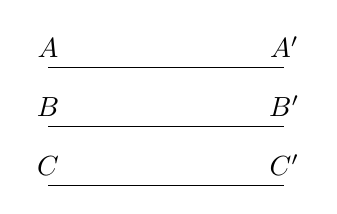
\begin{tikzpicture}[scale=0.75]
                              % Line for A--A'
                              \draw (0,0) -- (4,0);
                              \node[above]  at (0,0)   {$A$};
                              \node[above] at (4,0)   {$A'$};
                            
                              % Line for B--B'
                              \draw (0,-1) -- (4,-1);
                              \node[above]  at (0,-1)  {$B$};
                              \node[above] at (4,-1)  {$B'$};
                            
                              % Line for C--C'
                              \draw (0,-2) -- (4,-2);
                              \node[above]  at (0,-2)  {$C$};
                              \node[above] at (4,-2)  {$C'$};
                            \end{tikzpicture}
                        \end{center}
                        
                        \vspace{1em}
    
                        From the line AA', let the segment AE be subtracted:
    
                        \begin{center}
                            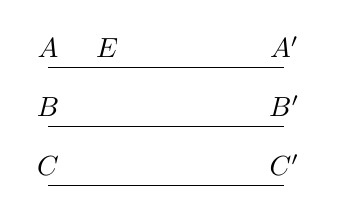
\begin{tikzpicture}[scale=0.75]
                              % A--E--A'
                              \draw (0,0) -- (4,0);
                              \node[above]  at (0,0)   {$A$};
                              \node[above] at (1,0)   {$E$};  % Place E somewhere between A and A'
                              \node[above] at (4,0)   {$A'$};
                            
                              % B--B'
                              \draw (0,-1) -- (4,-1);
                              \node[above]  at (0,-1)  {$B$};
                              \node[above] at (4,-1)  {$B'$};
                            
                              % C--C'
                              \draw (0,-2) -- (4,-2);
                              \node[above]  at (0,-2)  {$C$};
                              \node[above] at (4,-2)  {$C'$};
                            \end{tikzpicture}
                        \end{center}
                        
                        \vspace{1em}
    
                        and the segment CD added to the line CC', so that the whole line DCC' exceeds the line EA' by the segment CD and the segment CF; thus it exceeds the line BB' by the segment CD.
    
                        \begin{center}
                            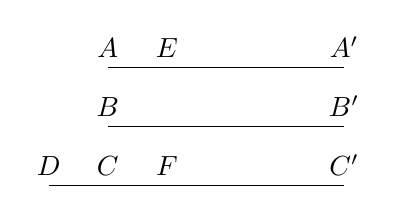
\begin{tikzpicture}[scale=0.75]
                              % A--E--A'
                              \draw (0,0) -- (4,0);
                              \node[above]  at (0,0)   {$A$};
                              \node[above] at (1,0)   {$E$};
                              \node[above] at (4,0)   {$A'$};
                            
                              % B--B'
                              \draw (0,-1) -- (4,-1);
                              \node[above]  at (0,-1)  {$B$};
                              \node[above] at (4,-1)  {$B'$};
                            
                              % D--C--F--C'
                              \draw (-1,-2) -- (4,-2);
                              \node[above]  at (-1,-2)  {$D$};
                              % Choose positions for C and F
                              \node[above] at (0,-2)  {$C$}; 
                              \node[above] at (1,-2)  {$F$};
                              \node[above] at (4,-2)  {$C'$};
                            \end{tikzpicture}
                        \end{center}
                        
                    \end{example}

\newpage

            \subsection{Two Kinds of Justice}

                \begin{definition}
                    \textbf{Distributive Justice} (Geometrical Proportion)
                    \begin{itemize}
                      \item Involves \textit{unequal} people (e.g., differing in merit) who should receive \textit{unequal} shares in proportion to their respective deserts.
                      \item Formula: $A : B = C : D$.
                    \end{itemize}
                \end{definition}

                \begin{definition}
                    \textbf{Rectificatory Justice} (Arithmetical Proportion)
                    \begin{itemize}
                      \item Involves \textit{equal persons} under the law who must be restored to a fair baseline when an injustice has occurred.
                      \item The judge ``corrects'' or ``rectifies'' by \textbf{subtracting} from the wrongdoer's gain and \textbf{adding} to the victim's loss.
                    \end{itemize}
                \end{definition}

                \subsubsection{Loss and Gain (revisited)}

                    \begin{itemize}
                      \item \textbf{Derivation}: The ideas of ``loss'' and ``gain'' come from \textit{voluntary exchange}, where one typically does not want to end up with less value (loss) or more than one's due (gain).
                      \item \textbf{Balance}: In just exchanges, each party ends with the value equivalent to what they began with, or at least with an agreed-upon equivalence of goods, services, or money.
                    \end{itemize}

            \subsection{Transactions}

                Aristotle divides transactions into:
                \begin{enumerate}
                  \item \textbf{Involuntary transactions}
                    \begin{itemize}
                      \item Examples: theft, assault, homicide, fraud, etc.
                      \item These necessitate the intervention of a judge or legal remedy to \textit{correct} (rectify) the imbalance.
                    \end{itemize}
                  \item \textbf{Voluntary transactions}
                    \begin{itemize}
                      \item Examples: commercial exchanges, renting, hiring, etc., where both parties consent.
                      \item These transactions \textit{can} still lead to disputes about ``gain'' and ``loss'' if the agreement is not honored or if one party defrauds the other.
                    \end{itemize}
                \end{enumerate}

                \subsubsection{Reciprocity}

                    Some philosophers (like the Pythagoreans) held that \textbf{reciprocity} (\emph{an eye for an eye}) is justice in an unqualified sense. However, Aristotle notes that strict reciprocity (literal tit-for-tat) does not accurately capture \textit{distributive} or \textit{rectificatory} justice, especially in cases where the parties' status is not the same (e.g., a citizen striking a magistrate might be punished more severely than if the roles were reversed).

                \subsubsection{Proportionate Reciprocation}\label{L1.2:Proportionate_Reciprocation}
                
                    Aristotle explains that in \textit{voluntary exchanges}, there is a form of justice he calls \textbf{``reciprocity in accordance with proportion.''} It is not mere equality of retaliation or transaction, but a reciprocal balance that accounts for the relative value of goods or services:
                    
                    \begin{quote}
                    If \textbf{A} is a builder and \textbf{B} is a shoemaker, and we want to exchange a house for shoes, the two must be \textit{commensurable} in a certain proportion so that the exchange is fair.
                    \end{quote}

        \section{A Third Kind of Justice}

            In addition to \textbf{distributive} and \textbf{rectificatory} justice, Aristotle explores a \textbf{third} concept often referred to as:
            \begin{quote}
            \[
            \text{\textit{antipeponthos kat' analogían}}
            \]
            \[
            \text{reciprocity in accordance with proportion.}
            \]
            \end{quote}

            This describes a kind of \textbf{proportional reciprocity} that arises especially in \textit{economic exchanges}, serving as the glue that holds a society together by rewarding good with good and returning bad with bad---yet doing so in proportion to the relative values or severity involved.

                \subsubsection{Proportionate Reciprocation}

                    When people engage in market exchanges, they must equate different goods in order to trade. Aristotle highlights:
                    \begin{itemize}
                      \item \textbf{A} (the builder)
                      \item \textbf{C} (a house)
                      \item \textbf{B} (the shoemaker)
                      \item \textbf{D} (shoes)
                    \end{itemize}

                    A fair exchange occurs when \textbf{A} receives from \textbf{B} a quantity of goods (shoes) that is proportionate in value to what \textbf{A} gives (a house). If one person's goods are inherently more valuable, the exchange ratio must reflect that.

            \subsection{Measure (The Role of Money)}

                Because houses, shoes, and other goods are not easily compared, society uses \textbf{money} as a conventional measure:
                \begin{enumerate}
                  \item Money acts as a \textbf{mean}, making goods and services \textbf{commensurable}.
                  \item It provides a universal measure of value so that we can compare ``how many shoes equal one house.''
                \end{enumerate}
                
                Aristotle derives the Greek word for money, \emph{nomisma}, from \textit{nomos} (law or convention), to emphasize that money's value is established by collective agreement. Without money, trade would rely on barter, which complicates finding fair ratios (how many shoes per house?).

                \subsubsection{Proportional Reciprocity in Practice}

                    It is not that two doctors exchange services, but rather a farmer and a doctor, or a builder and a shoemaker. Because these parties produce different and \textit{unequal} things, there must be a standardized method (money) to equate and balance their transactions. This fosters \textbf{social cohesion}: people exchange goods or services in proportion to their value, keeping relationships functional and the city unified.

        \section*{L1.2 -- Conclusions}

            Aristotle's discussion in Book V of the \textit{Nicomachean Ethics} reveals how \textbf{justice} can be understood in several overlapping senses:
            \begin{enumerate}
              \item \textbf{Distributive justice} deals with proportional allocations to \textbf{unequal} persons, according to their merit (geometrical proportion).
              \item \textbf{Rectificatory justice} addresses the correction of wrongs through \textbf{arithmetical} proportion, treating the parties as equals before the law, subtracting from the wrongdoer's excess and compensating the victim's loss.
              \item \textbf{Proportionate reciprocity} (sometimes taken as a \textbf{third} kind of justice) emphasizes fair exchange in economic or social transactions, achieved through a \textbf{proportional} equality rather than mere equality. Money becomes a key instrument for measuring and making commensurable the goods or services exchanged.
            \end{enumerate}
            
            \begin{remark}
                In \textbf{distributive} justice, differences in people's status or merit lead to \textbf{unequal} allocations that are still fair because they are \textit{proportionate}. In \textbf{rectificatory} justice, the parties are treated as \textbf{equals} in the sense that the law imposes a correction for the wrongdoing. In \textbf{exchange}, people's different products or services must be brought into a \textbf{proportionate} equality so that trade can occur fairly.
            \end{remark}

            \begin{remark}[Why we use mathematics in \ref{L1.2:Proportionate_Reciprocation}]
                From the greek ``\textit{mathēmatikē}'', from the base of ``\textit{manthanein}'', to learn. It is simply more logical to argue via the use of math, as it allows us to uncover and argue for something that is already known.
            \end{remark}
            
            Aristotle's overarching conclusion is that although all three share something in common---namely, the idea of \textbf{balance} or \textbf{mean}---they apply in different realms (distribution of public goods, correction of private harms, and exchange of goods/services). Where \textbf{distributive justice} and \textbf{rectificatory justice} ``rectify'' imbalances by either awarding shares in proportion to merit or compensating losses, \textbf{proportionate reciprocity} emphasizes mutual benefit and the cohesive power of fair trade in the city.
            
            Thus, differences are recognized---merit, wrongdoing, product value---but justice seeks to bring them into a \textbf{measured} or \textbf{proportional} equilibrium, preserving harmony and fairness in social life.


    \chapter[Just Price and Quantities of Labour]{Thomas Aquinas \\[0.6cm] \textit{Just Price and Quantities of Labour}}

        \section{\textit{Summa Theologiae}}

    \begin{remark}
        Thomas Aquinas’s discussion of \textit{just price} and related issues in buying and selling draws heavily on Aristotle’s works, most notably \textit{Politics} (Book I) and \textit{Nicomachean Ethics} (Book V). It also engages with classical examples provided by Cicero (e.g., \textit{De Officiis}) and relies on Roman law regarding contracts and fairness (\textit{Codex Iustinianus}).
    \end{remark}

    \subsection{Question 77: On cheating in buying and selling}

        \subsubsection{Article 3. Whether the seller is bound to state the defects of the thing sold}

            \begin{quote}
                Suppose, for example, a time of dearth and famine at Rhodes, with provisions at fabulous prices; and suppose that an honest man has imported a large cargo of grain from Alexandria and that to his certain knowledge also several other importers have set sail from Alexandria, and that on the voyage he has sighted their vessels laden with grain and bound for Rhodes; is he to report the fact to the Rhodians or is he to keep his own counsel and sell his own stock at the highest market price?
            
                (Cicero, \textit{De Officiis}, Book 3.50)
            \end{quote}
    
            \begin{quote}
                [...] it is not in accord with Nature that anyone should take advantage of his neighbour’s ignorance.
            
                (Cicero, \textit{De Officiis}, Book 3.72)
            \end{quote}
    
            Aquinas distinguishes between hiding an actual, present defect in goods versus simply withholding information about future events. A defect in a thing lessens its value \emph{in the present}, while in the Rhodes example the coming arrival of additional grain will lessen the price \emph{in the future}. Since future circumstances are by definition uncertain to the buyer, Aquinas holds that the seller who sells at the current market price does not commit an injustice merely by not revealing the future influx of grain. He does acknowledge that revealing such information or voluntarily lowering the price would be more virtuous, but it is not strictly required by justice.
    
            \begin{quote}
                \textit{Ad quartum dicendum quod vitium rei facit rem in praesenti esse minoris valoris quam videatur, sed in casu praemisso, in futurum res expectatur esse minoris valoris per superventum negotiatorum, qui ab ementibus ignoratur. Unde venditor qui vendit rem secundum pretium quod invenit, non videtur contra iustitiam facere si quod futurum est non exponat. Si tamen exponeret, vel de pretio subtraheret, abundantioris esset virtutis, quamvis ad hoc non videatur teneri ex iustitiae debito.}
            \end{quote}
    
            \begin{remark}
            Aquinas concludes that such a situation is \emph{not} a fraud in the strict sense but rather a change in circumstance (present vs.\ future). In other words, if the item truly has a defect in the here and now, the seller is obliged to disclose it; if the expected lowering of the price is only in the future, one is not strictly obligated to mention it.
            \end{remark}
    
            Aquinas also draws on Aristotle’s principle that transactions \emph{ought} to observe an “equality of thing and thing.” Yet, in practical realities, exceptions may occur without constituting injustice.

        \subsubsection{Article 4. Whether, in trading, it is licit to sell a thing at a higher price than what was paid for it}

            \begin{quote}
                A tradesman is one whose business consists in the exchange of things. According to the Philosopher (Polit. i, 3), exchange of things is twofold: one, natural as it were, and necessary, whereby one commodity is exchanged for another, or money taken in exchange for a commodity, in order to satisfy the needs of life. Such like trading, properly speaking, does not belong to tradesmen, but rather to housekeepers or civil servants who have to provide the household or the state with the necessaries of life. 
            
                The other kind of exchange is either that of money for money, or of any commodity for money, not on account of the necessities of life, but for profit, and this kind of exchange, properly speaking, regards tradesmen, according to the Philosopher (Polit. i, 3). The former kind of exchange is commendable because it supplies a natural need: but the latter is justly deserving of blame, because, considered in itself, it satisfies the greed for gain, which knows no limit and tends to infinity.
            \end{quote}

            Aquinas remarks that trading for profit \emph{by itself} does not necessarily entail sinfulness, provided the intention is just. It becomes permissible if one’s ultimate goal is, for example, the upkeep of one’s household or the relief of the poor, rather than an endless accumulation of wealth. In such cases, a markup can be seen as “\textit{stipendium laboris},” i.e., compensation for labor, transport, or risk.

            \begin{quote}
                Hence trading, considered in itself, has a certain debasement attaching thereto, in so far as, by its very nature, it does not imply a virtuous or necessary end. Nevertheless gain which is the end of trading, though not implying, by its nature, anything virtuous or necessary, does not, in itself, connote anything sinful or contrary to virtue: wherefore nothing prevents gain from being directed to some necessary or even virtuous end, and thus trading becomes licit. [...] For if he sells at a higher price something that has changed for the better, he would seem to receive the reward of his labour.
            \end{quote}

            The key point is that if the item truly \emph{increases in value}—either because of the labor expended in improving it, or because of the costs (danger, transportation, etc.) involved—charging a higher price is legitimate and does not violate justice.

    \subsection{Question 61: The parts of Justice}

        Aquinas notes that Aristotle, in \textit{Nicomachean Ethics} Book V, distinguishes two basic forms of justice:
        \begin{enumerate}
            \item \textbf{Distributive justice}, whose mean is determined by \emph{geometrical proportion}. Those who are more “worthy” (e.g., possessing higher rank, ability, or contribution to the common good) receive proportionally more from the common stock.
            \item \textbf{Commutative (or Corrective) justice}, whose mean is determined by \emph{arithmetical proportion}. This applies to voluntary exchanges (like buying and selling) or involuntary exchanges (like theft or violence). Here we do not weigh personal status but rather strictly ensure that each party receives or restores an amount equal to what was lost or gained.
        \end{enumerate}

        \begin{quote}
            The Philosopher says (Ethic. v, 3,4) that the mean in distributive justice is observed according to ``geometrical proportion,'' whereas in commutative justice it follows “arithmetical proportion.” [...]
            
            On the other hand, in commutations something is paid to an individual on account of something of his that has been received [...] Hence it is necessary to equalize thing with thing, so that the one person should pay back to the other just so much as he has become richer out of that which belonged to the other. [...]
        \end{quote}

        \begin{remark}
            Aquinas \emph{collapses} many possible distinctions of exchange (including punitive “contrapassum”) into commutative justice. This allows a judge or an authority, if needed, to impose restitution or compensation and thereby restore equality.
        \end{remark}

        He also explains the notion of \emph{reciprocity} (\textit{contrapassum}), i.e.\ returning harm for harm, or restitution for what was taken:
        
        \begin{quote}
            Reciprocity [\textit{contrapassum}] denotes equal passion repaid for previous action; and the expression applies most properly to injurious passions and actions, whereby a man harms the person of his neighbor; for instance if a man strike, that he be struck back. [...] And since also to take away what belongs to another is to do an unjust thing, it follows that secondly reciprocity consists in this also, that whosoever causes loss to another, should suffer loss in his belongings, [...]. 
        \end{quote}
        
        Yet perfect equality is not always straightforward: striking a mere citizen versus striking a prince, for example, might receive different punishments to maintain the proportional or corrective “mean.” Likewise, theft or fraud in property may be punished by returning more than the stolen value, taking into account the harm to the wider community.

    \subsection*{Back to Question 77: On cheating in buying and selling}

        \subsubsection{Article 1. Whether it is licit to sell a thing for more than its value}

            Aquinas clarifies that employing deceit is always sinful. But absent deceit, there are two main considerations:
            
            \begin{enumerate}
                \item \emph{Buying and selling considered in themselves}. In principle, exchange is for the mutual advantage of both parties. This requires an equality of “thing and thing” and the avoidance of exploitation. Money was introduced exactly to measure this equivalence. If the \emph{price} unreasonably exceeds the \emph{thing’s value} (or vice versa), it violates commutative justice.
            
                \item \emph{Buying and selling considered in relation to special circumstances}. For instance, if the seller will incur a particular \emph{loss} or bears certain costs or risks, the “just price” can rightly be higher. Thus Aquinas allows selling at a higher price if that higher price genuinely reflects additional expenses, risks, or the utility the buyer personally attributes to the good.
            \end{enumerate}
            
            He also references how different legal or moral systems might respond. \emph{Human law} may tolerate certain lesser injustices and only punish more egregious ones (e.g., cases involving an overcharge greater than half the thing’s value, referencing Roman law on \textit{laesio enormis}). \emph{Divine law}, on the other hand, leaves nothing unpunished that is contrary to virtue. 

            \begin{quote}
                Accordingly, if without employing deceit the seller sells his goods overvaluing them (\textit{rem suam supervendat}), or the buyer obtain them for less, the law looks upon this as licit, and provides no punishment for so doing, unless the excess be too great, because then even human law demands restitution to be made [...]. 
                
                On the other hand, the Divine law leaves nothing unpunished that is contrary to virtue. [...] I add this condition, because the just price of things (\textit{iustum pretium rerum}) is not precisely determined (\textit{non est punctualiter determinatum}), but consists in a kind of estimate (\textit{in quadam aestimatione consistit}), so that a slight addition or subtraction would not seem to destroy the equality of justice.
            \end{quote}
            
            In other words, prices often involve an \emph{estimate} (because the “exact” value of a thing can be hard to establish). So minor deviations need not be considered injustice, but significant deviations may require restitution.

\section{Commentary on Aristotle's \textit{Nicomachean Ethics}}

    Aquinas’s \textit{Commentary on the Nicomachean Ethics} further discusses how just exchange depends on proportional equivalences:
    
    \begin{quote}
        971. Next […], he [Aristotle] explains in what matter and manner the statement is true that reciprocation is justice. He discusses this point from three aspects. First [III, A] he shows that there must be reciprocation in exchanges according to proportionality. Then […], he explains the form of this proportionality. Last [Lect. 9; C], at “Therefore all etc.” (B. 1133 a 18), he shows how such a form can be observed. […] He says that in dealings of exchange it is true that justice is of such a nature that it includes reciprocation not according to equality but according to proportionality.
    \end{quote}
    
    \begin{quote}
        972. It seems this is contrary to what was said before (950), that in commutative justice the mean is taken not according to geometrical proportionality, which consists in an equality of proportion, but according to arithmetic proportionality, which consists in a quantitative equality. We must say that, in regard to commutative justice there should always be an equality of thing to thing, not, however, of action and passion, which implies corresponding requital. But in this, proportionality must be employed in order to bring about an equality of things because the work of one craftsman is of more value than the work of another, e.g., the building of a house than the production of a penknife. Hence, if the builder exchanged his work for the work of the cutler, there would not be equality of thing, given and taken, i.e., of house and penknife.
    \end{quote}

    Here, Aquinas’s point (following Aristotle) is that \emph{some} form of proportional balancing is needed so that, for example, the combined labor or value put into \emph{many} sandals might properly match the labor or value of building a \emph{house}. Strict one-for-one exchange of different goods could be obviously unfair.

    \begin{quote}
        980. Next […], he shows how exchange takes place according to the preceding commensuration. Although a house is worth more than a sandal, nevertheless, a number of sandals are equal in value to one house or the food required for one man during a long period. [...] If this is not observed, there will be no exchange of things and men will not share their goods with one another.
    \end{quote}
    
    \begin{quote}
        983. Then […], he shows how just reciprocation takes place in exchanges according to the preceding commensuration. [...] He says first that the norm measuring all things by need according to nature and by currency according to human convention will then become reciprocation when everything will be equated in the way just mentioned.
    \end{quote}
    
    Aquinas explains Aristotle’s use of a “proportional figure with diagonals”—the well-known schematic in Book V of the \textit{Nicomachean Ethics}—to illustrate how different trades and values must be matched in some ratio. If the builder invests more labor or expense, that difference should be compensated by a correspondingly larger quantity of goods from the other party.

    \begin{quote}
        Thus, when exchange of things (\textit{commutatio rerum}) takes place, the articles to be exchanged (\textit{res commutandas}) ought to be arranged in a proportional figure with diagonals, as was stated previously (957). If this was not done, one extreme would have both excesses (\textit{superabundantias});
    
        if a farmer gave a bushel of wheat for a sandal, he would have an excess of labour in his product (\textit{superabundantiam laboris in opere}) and would have also an excess of presents (\textit{superabundantiam doni}) because he would be giving more than he would receive. But when all have what is theirs, they are in this way equal and do business with one another because the equality previously mentioned is possible for them.
    \end{quote}

\section*{Additional Context and Observations}

    \begin{remark}[Roman Law and the “Just Price”]
        Aquinas’s notion of \emph{just price} was influenced by Roman legal principles, such as those found in the \textit{Codex Iustinianus}. One doctrine, \textit{laesio enormis}, allowed a contract to be rescinded if it was made at less than half of the fair market value. Aquinas often reconciles such legal norms with moral theology: human law tolerates smaller deviations but punishes larger ones.
    \end{remark}

    \begin{remark}[Moral vs. Legal Dimensions]
        Aquinas’s distinction between the requirements of \emph{human law} and \emph{divine law} underscores that, from the standpoint of perfect virtue, even smaller injustices in exchange can be blameworthy. However, civil law ordinarily penalizes only the more severe cases so that social order remains manageable among “many lacking in virtue.”
    \end{remark}

    \begin{remark}[Natural vs. Unnatural Exchange (Aristotle’s Framework)]
        Following Aristotle, Aquinas differentiates between (a) \emph{natural exchange}, which serves to provide for genuine needs (e.g., household provisioning) and is seen as ethically commendable, and (b) \emph{unnatural or artificial exchange}, which solely pursues profit or speculation. This latter is neither intrinsically sinful nor virtuous but can become morally questionable when it stems from greed or exploits others.
    \end{remark}

    \begin{remark}[Labour, Risk, and Transportation]
        Aquinas consistently holds that a higher selling price may be justified when it compensates for improvements, labour, transport costs, or risk borne by the merchant. Thus, “buying low and selling high” is not automatically unjust; it depends on whether the markup is proportionate to real added value or costs.
    \end{remark}

    \begin{remark}[Practical Applicability]
        Although Aquinas lived in a medieval context (13th century), his arguments about honesty in trade, transparency of defects, and fairness in pricing remain influential in discussions of market ethics, consumer protection, and economic justice today.
    \end{remark}

        \subsubsection{Final considerations}

    \noindent In summary, Aquinas’s teaching on just price centres on the principle that transactions must preserve a certain equality, measured not only by the intrinsic worth of the item but also by factors such as labour input, risk undertaken, and legitimate need of both parties. While human law may choose to tolerate minor deviations from perfect equity, moral theology requires that all intentional distortion or fraud be avoided. Exchanges should, as far as possible, reflect a mutual benefit and fair equivalence between what is given and what is received—a principle that finds its roots in both Aristotelian philosophy and the broader Christian moral tradition.


    \chapter[Survival and the state of nature]{Thomas Hobbes \\[0.6cm] \textit{Survival and the state of nature}}

        \subsection*{Historical Context}

        \begin{itemize}
            \item \textbf{Protestant Reformation (1517)}
            \begin{itemize}
                \item Initiated by Martin Luther, leading to significant religious and political upheaval in Europe.
                \item Contributed to the fragmentation of the Catholic Church and fueled inter-state and intra-state conflicts.
            \end{itemize}
        
            \item \textbf{European Religious Wars (16th--17th centuries and beyond)}
            \begin{itemize}
                \item Culmination of tensions between Protestants and Catholics.
                \item These conflicts ravaged many European regions, fostering an environment of mistrust, instability, and the need for strong governance.
            \end{itemize}
        
            \item \textbf{Scientific Revolution: Galileo (1564--1642), Descartes (1596--1650)}
            \begin{itemize}
                \item A shift toward empiricism and rational inquiry.
                \item Galileo’s emphasis on observation and mathematics, and Descartes’ focus on methodic doubt and the primacy of reason, challenged traditional Scholastic frameworks in philosophy and natural science.
            \end{itemize}
        
            \item \textbf{English Civil War (1642--1651)}
            \begin{itemize}
                \item Fought between Royalists (supporters of King Charles I) and Parliamentarians (supporters of parliamentary power).
                \item Thomas Hobbes lived through this period of turmoil. His experiences informed his conviction that strong central authority is necessary to prevent chaos.
            \end{itemize}
        \end{itemize}
        
        These historical factors deeply influenced Hobbes’s thinking. The \textit{Protestant Reformation} and the ensuing religious wars showed him how divergent beliefs can destabilize entire societies, while the \textit{Scientific Revolution} shaped his mechanical, materialist approach to human cognition and social organization. The immediate political unrest of the \textit{English Civil War} offered him a firsthand example of the dangers of insufficiently centralized power.

\section{\textit{Leviathan} (1651)}

    Thomas Hobbes’s Leviathan is one of the foundational texts of modern political philosophy. Published amidst the chaos of the English Civil War, it offers a rigorous defense of absolute sovereignty as a means to ensure peace and security. Before discussing the notion of the commonwealth, Hobbes establishes the philosophical basis of his approach by explaining his conception of sense, imagination, and the motions that drive human passions.

        \subsubsection{The origin of our thoughts}

            \begin{quote}
                Concerning the thoughts of man, I will consider them first singly, and afterwards in train or dependence upon one another. Singly, they are every one a representation or appearance of some quality, or other accident of a body without us, which is commonly called an object. Which object worketh on the eyes, ears, and other parts of man’s body, and by diversity of working produceth diversity of appearances.  The original of them all is that which we call SENSE, (for there is no conception in a man’s mind which hath not at first, totally or by parts, been begotten upon the organs of sense). The rest are derived from that original. 
            \end{quote} 

            Hobbes begins by describing thought and consciousness as fundamentally connected to sense experience. For him, all cognition—every idea, concept, or thought—can be traced back to an external object pressing upon our sensory organs. This “pressing” or “motion” triggers internal changes that we register as sense impressions.

            \begin{remark}
                There is no content in the mind that did not first originate in sense (a direct challenge to the idea of innate knowledge). Thought builds upon and rearranges these original sensory inputs over time.
            \end{remark}

        \subsubsection{The cause of sense}

            \begin{quote}
                The cause of sense is the external body, or object, which presseth the organ proper to each sense, either immediately, as in the taste and touch; or mediately, as in seeing, hearing, and smelling: which pressure, by the mediation of nerves and other strings and membranes of the body, continued inwards to the brain and heart, causeth there a resistance, or counter-pressure (anti-tupia), or endeavour of the heart to deliver itself: which endeavour, because outward, seemeth to be some matter without.
            \end{quote}

            For Hobbes, sense arises through a mechanical process: external objects literally press upon our sense organs (directly for taste and touch, or indirectly for vision and hearing), causing a chain reaction of motions. Hobbes is adopting the nascent mechanical philosophy of his era, influenced by thinkers like Galileo, who emphasized that all observable phenomena (including perception) can be explained in terms of matter and motion.

\newpage
        \subsubsection{Several motions of the matter}

            \begin{quote}
                And this seeming, or fancy, is that which men call sense; and consisteth, as to the eye, in a light, or colour figured; to the ear, in a sound; to the nostril, in an odour; to the tongue and palate, in a savour; and to the rest of the body, in heat, cold, hardness, softness, and such other qualities as we discern by feeling. All which qualities called sensible are in the object that causeth them but so many several motions of the matter, by which it presseth our organs diversely. Neither in us that are pressed are they anything else but diverse motions (for motion produceth nothing but motion).
            \end{quote}

            Here, Hobbes extends this mechanical explanation to clarify that what we perceive as “heat,” “cold,” “color,” or “sound” is actually the effect of various motions in objects interacting with our organs. The “qualities” we perceive—like color—are not identical to anything literally colored existing outside us, but rather the result of our nervous system’s interpretation of motion.

            In modern philosophy, this distinction is sometimes referred to as the difference between:

            \begin{itemize}
                \item \textbf{Primary qualities} (e.g., extension, motion) which inhere in objects themselves.
                \item \textbf{Secondary qualities} (e.g., color, taste, sound) which are the mind’s interpretation of those motions.
            \end{itemize}

        \subsubsection{The object is one thing, the image is another}

            \begin{quote}
                But their appearance to us is fancy, the same waking that dreaming. And as pressing, rubbing, or striking the eye makes us fancy a light, and pressing the ear produceth a din; so do the bodies also we see, or hear, produce the same by their strong, though unobserved action…

                And though at some certain distance the real and very object seem invested with the fancy it begets in us; yet still the object is one thing, the image or fancy is another. So that sense in all cases is nothing else but original fancy caused (as I have said) by the pressure that is, by the motion of external things upon our eyes, ears, and other organs, thereunto ordained.
            \end{quote}

            This underlines Hobbes’s representational theory of perception: there is always a distinction between the external thing and the mental image or representation we have of it. He emphasizes that the process by which we see or hear something resembles the effect of physically pressing upon the relevant sense organ.

    \subsection[Of Sense]{Chapter 1 \\ \textit{Of Sense}}

        \begin{remark}
            \begin{itemize}
                \item The origin of thought is sense.
                \item The origin of sense is an impression of an external object.
                \item Sense is an appearance that does not coincide with the object that caused it.
            \end{itemize}
        \end{remark}

        \subsubsection{Opposition to Scholasticism}

            \begin{quote}
                But the philosophy schools, through all the universities of Christendom, grounded upon certain texts of Aristotle, teach another doctrine; and say, for the cause of vision, that the thing seen sendeth forth on every side a visible species, (in English) a visible show, apparition, or aspect, or a being seen; the receiving whereof into the eye is seeing. And for the cause of hearing, that the thing heard sendeth forth an audible species, that is, an audible aspect, or audible being seen; which, entering at the ear, maketh hearing. Nay, for the cause of understanding also, they say the thing understood sendeth forth an intelligible species, that is, an intelligible being seen; which, coming into the understanding, makes us understand.

                I say not this, as disapproving the use of universities: but because I am to speak hereafter of their office in a Commonwealth, I must let you see on all occasions by the way what things would be amended in them; amongst which the frequency of insignificant speech is one.
            \end{quote}

            Hobbes rejects the Scholastic notion of “species” or “forms” emanating from objects. According to the Aristotelian tradition, a “visible species” travels to our eyes, or an “audible species” reaches our ears. Hobbes sees these explanations as outdated and unnecessarily obscure, preferring instead a mechanistic, matter-in-motion account of perception.

    \subsection*{Digression: Artistotle}

        \begin{remark}
            There is not just one pressure or external force, but two, two powers, or better, two capacities, two dispositions: \textit{dynamis} (dynamism, movement, tension)

            The meeting of two dispositions: \textit{energheia} (energy), the accomplishment
        \end{remark}

        \subsubsection{Aesthetics (Aisthesis)}

            From the viewpoint of sensing (aisthesis):

            \begin{enumerate}
                \item Two dynamis:
                    \begin{itemize}
                        \item The table has the capacity or disposition to be seen.
                        \item I have the capacity or disposition to see.
                    \end{itemize}
                \item Energeia:
                    \begin{itemize}
                        \item When these capacities meet, I actually see the table, and the table is seen.
                    \end{itemize}
            \end{enumerate}

        \subsubsection{Technique}

            From the point of view of the techné (technique): 

            \begin{itemize}
                \item \textbf{Two dynamis}: the capacity of the table to be used (it is ready to be used), my capacity to use it
                \item \textbf{Energheia}: I use the table and the table is used by me
            \end{itemize}

            \begin{example}[Capacities and Use]
                Similarly, a table can be used, and a person has the capacity to use it. When these capacities come together, the object’s purpose (\textit{telos}) is realized—“the table is used.”
            \end{example}

            From Aristotle to Aquinas to Hobbes:
            
            \begin{itemize}
                \item \textbf{Aristotle \& Aquinas}: potentia (dynamis) vs. actus (energheia).
                \item \textbf{Hobbes}: Replaces these more “metaphysical” accounts with physical “motion of matter.”
            \end{itemize}

    \subsection[Of Imagination]{Chapter 2 \\ \textit{Of Imagination}}

        \subsubsection{Inertia}

            \begin{quote}
                That when a thing lies still, unless somewhat else stir it, it will lie still for ever, is a truth that no man doubts of. But that when a thing is in motion, it will eternally be in motion, unless somewhat else stay it, though the reason be the same (namely, that nothing can change itself), is not so easily assented to.
            \end{quote}

            Reflecting the post-Galilean world, Hobbes applies the principle of inertia to mental phenomena. Just as a physical object stays in motion unless stopped, an impression in the mind persists (as imagination) after the initial sensory input is removed.

    \subsection[Of the Interior Beginnings of Voluntary Motions, commonly called Passions]{Chapter 6 \\ \textit{Of the Interior Beginnings of Voluntary Motions, commonly called Passions}}

        \subsubsection{Vital and animal motion}

            \begin{quote}
                There be in animals two sorts of motions peculiar to them: One called vital, begun in generation, and continued without interruption through their whole life; such as are the course of the blood, the pulse, the breathing, the concoction, nutrition, excretion, etc.; to which motions there needs no help of imagination: the other is animal motion, otherwise called voluntary motion; as to go, to speak, to move any of our limbs, in such manner as is first fancied in our minds. That sense is motion in the organs and interior parts of man’s body, caused by the action of the things we see, hear, etc., and that fancy is but the relics of the same motion, remaining after sense, has been already said in the first and second chapters.
            \end{quote} 

            \begin{itemize}
                \item \textbf{Vital Motions}: Automatic bodily functions (heartbeat, digestion, breathing).
                \item \textbf{Animal (Voluntary) Motions}: Motions directed by conscious thought, e.g., walking, speaking, grasping an object.
            \end{itemize}

        \subsubsection{Small beginnings of motion}

            \begin{quote}
                And because going, speaking, and the like voluntary motions depend always upon a precedent thought of whither, which way, and what, it is evident that the imagination is the first internal beginning of all voluntary motion. And although unstudied men do not conceive any motion at all to be there, where the thing moved is invisible, or the space it is moved in is, for the shortness of it, insensible; yet that doth not hinder but that such motions are. For let a space be never so little, that which is moved over a greater space, whereof that little one is part, must first be moved over that. These small beginnings of motion within the body of man, before they appear in walking, speaking, striking, and other visible actions, are commonly called endeavour.
            \end{quote}

            \begin{itemize}
                \item \textbf{Precedent Thought}: Before any visible action (speaking, moving a limb), there is a “small,” internal motion in the mind—an endeavour or conatus.
                \item \textbf{Invisible Steps}: Hobbes highlights that even seemingly instantaneous decisions involve a micro-phase of mental motion that initiates the physical act.
            \end{itemize}

        \subsubsection{\textit{Conatus}}

            This endeavour (\textit{conatus}), when it is toward something which causes it, is called appetite, or desire, the latter being the general name, and the other oftentimes restrained to signify the desire of food, namely hunger and thirst. And when the endeavour is from ward something, it is generally called aversion.

            \begin{itemize}
                \item \textbf{Appetite} (Desire) vs. \textbf{Aversion}: If the mental motion is directed toward something, it is desire; if away, it is aversion.
                \item \textbf{Mechanistic Emotion}: Hobbes “mechanizes” the passions, framing even desire and fear as motions—pushing us either to approach or to retreat.
            \end{itemize}

    \subsection[Of the Difference of Manners]{Chapter 9 \\ \textit{Of the Difference of Manners}}

        \subsubsection{Felicity is not satisfaction}

            \begin{quote}
                By manners, I mean not here decency of behaviour; as how one man should salute another, or how a man should wash his mouth, or pick his teeth before company, and such other points of the small morals; but those qualities of mankind that concern their living together in peace and unity. To which end we are to consider that the felicity of this life consisteth not in the repose of a mind satisfied. For there is no such finis ultimus (utmost aim) nor summum bonum (greatest good) as is spoken of in the books of the old moral philosophers. Nor can a man any more live whose desires are at an end than he whose senses and imaginations are at a stand. Felicity is a continual progress of the desire from one object to another, the attaining of the former being still but the way to the latter.
            \end{quote}

            \begin{itemize}
                \item \textbf{No Ultimate End}: Rejects the ancient idea of a highest good (summum bonum). Humans never reach a point of permanent fulfillment; desire pushes us ceaselessly onward.
                \item \textbf{Restless Pursuit}: This perpetual seeking clarifies why humans strive for power and resources—there is no static state of contentment.
            \end{itemize}

        \subsubsection{A restless desire of power after power}

            \begin{quote}
                So that in the first place, I put for a general inclination of all mankind a perpetual and restless desire of power after power, that ceaseth only in death… because he cannot assure the power and means to live well, which he hath present, without the acquisition of more.
                
                Desire of ease, and sensual delight, disposeth men to obey a common power.
            \end{quote}

            \begin{itemize}
                \item \textbf{Security and Survival}: Hobbes traces our thirst for power to anxiety about our safety and well-being. We seek more power to ensure our current power is not undermined by others.
                \item \textbf{Roots of Conflict}: This universal drive can lead to competition and conflict. However, it also motivates people to accept a common power that can ensure they will not be harmed by rivals.
            \end{itemize}

    \subsection[Of the Natural Condition of Mankind as concerning their Felicity and Misery]{Chapter 13 \\ \textit{Of the Natural Condition of Mankind as concerning their Felicity and Misery}}

        \subsubsection{Diffidence of one another}

            \begin{quote}
                [...] if one plant, sow, build, or possess a convenient seat, others may probably be expected to come prepared with forces united to dispossess and deprive him, not only of the fruit of his labour, but also of his life or liberty.
            \end{quote}

            \begin{remark}[State of nature]
                Hobbes describes a scenario where there is no common power—no government, no laws, no shared enforcement mechanisms. In such a situation, trust is low, and the fear of losing one’s possessions (and life) is high.
            \end{remark}

        \subsubsection{Anticipation}

            \begin{quote}
                And from this diffidence of one another, there is no way for any man to secure himself so reasonable as anticipation; that is, by force, or wiles, to master the persons of all men he can so long till he see no other power great enough to endanger him: and this is no more than his own conservation requireth, and is generally allowed.
            \end{quote}

            \begin{proposition}[Preemptive Strikes]
                Feeling threatened, individuals may resort to attacking others first. This is deemed rational in the absence of a higher authority to guarantee safety.
            \end{proposition}

        \subsubsection{War against all}

            \begin{quote}
                Hereby it is manifest that during the time men live without a common power to keep them all in awe, they are in that condition which is called war; and such a war as is of every man against every man. For war consisteth not in battle only, or the act of fighting, but in a tract of time, wherein the will to contend by battle is sufficiently known: and therefore the notion of time is to be considered in the nature of war, as it is in the nature of weather. For as the nature of foul weather lieth not in a shower or two of rain, but in an inclination thereto of many days together: so the nature of war consisteth not in actual fighting, but in the known disposition thereto during all the time there is no assurance to the contrary. All other time is peace.
            \end{quote}

            \begin{itemize}
                \item \textbf{Definition of War}: War is not just combat but the known disposition to fight—an enduring state of suspicion and readiness to clash.
                \item \textbf{Time and Fear}: Just as “foul weather” involves an ongoing threat of storms, so “war” is a persistent threat of violence when no one can be sure of security.
            \end{itemize}

\section{\textit{Homo Homini Lupus}}

        \subsubsection{No place for industry}

            \begin{quote}
                In such condition there is no place for industry, because the fruit thereof is uncertain: and consequently no culture of the earth; no navigation, nor use of the commodities that may be imported by sea; no commodious building; no instruments of moving and removing such things as require much force; no knowledge of the face of the earth; no account of time; no arts; no letters; no society; and which is worst of all, continual fear, and danger of violent death; and the life of man, solitary, poor, nasty, brutish, and short.
            \end{quote}

            \begin{remark}[Consequences of Anarchy]
                 In this Hobbesian “state of nature,” the lack of security stifles all productive or cooperative pursuits—farming, trade, the arts, and science cannot flourish under constant fear of attack.
            \end{remark}

        \subsubsection{No pleasure in keeping company}

            \begin{quote}
                Again, men have no pleasure (but on the contrary a great deal of grief) in keeping company where there is no power able to overawe them all.
            \end{quote}

            \begin{itemize}
                \item \textbf{Human Beings as Antisocial by Nature}: Here, Hobbes rejects the Aristotelian idea that “man is by nature a political animal” (zoon politikon). Instead, absent an overawing power, humans are driven apart by mutual distrust.
                \item \textbf{Civil State as a Solution}: Ironically, it is precisely our antisocial self-interest—the fear of others’ aggression—that compels us to seek peace under a common authority (the Leviathan).
            \end{itemize}

    \begin{remark}
        Human being is neither a \textit{zoon politikon} nor an \textit{animal sociale}

        In the state of nature, human beings are antisocial

        But it is the antisocial principle (the fear of others’ fear) that brings them together in the civil state (under a common power)
    \end{remark}

\section*{Additional Context and Observations}

    \begin{remark}[Hobbes’s Biographical Context]
        He was tutored in classical languages, worked as a secretary and companion to noble families, and mingled with leading intellectuals in France and England. This shaped his blending of classical scholarship with cutting-edge scientific theory.
    \end{remark}

    \begin{remark}[Religious Overtones]
        Despite championing a materialist account, Hobbes was wary of being branded irreligious. He devotes substantial portions of Leviathan to scriptural interpretation, aiming to reconcile his political conclusions with a Christian framework.
    \end{remark}

    \begin{remark}[Comparison with Other Social Contract Theorists]
        Later writers (Locke, Rousseau, Kant) adopt the idea of a social contract but often reject Hobbes’s pessimistic anthropology. They propose that certain natural rights (e.g., property, liberty) must remain inalienable.
    \end{remark}

    \begin{remark}[Hobbes and Geometry]
        Hobbes fancied himself a geometer and believed that the clarity of geometric demonstration could be applied to moral and political philosophy. While he was not always successful in advanced geometry, this aspiration shaped his methodical presentation.
    \end{remark}

    \subsection*{Final Considerations}

        Hobbes’s Leviathan culminates in a social contract theory: individuals in the state of nature, driven by fear and rational self-interest, agree to yield their individual rights to a sovereign power in exchange for peace and security. This sovereign (whether a monarch or an assembly) must be all-powerful, otherwise it cannot enforce the peace effectively. Hobbes’s choice of the biblical sea monster “Leviathan” as a metaphor underscores the intimidating might required to compel obedience and protect subjects from each other.

        \begin{itemize}
            \item \textbf{Influence on Modern Political Thought}: Hobbes’s work laid a foundation for later contract theorists like John Locke and Jean-Jacques Rousseau, though they often took a more optimistic view of human nature.
            \item \textbf{Mechanical Materialism}: Hobbes extended the logic of the Scientific Revolution to explain both human cognition and social organization in terms of motion, pressure, and mechanistic causation.
            \item \textbf{Critiques and Legacy}: Critics argue Hobbes undervalues moral, spiritual, or civic virtues beyond self-preservation. Nonetheless, Leviathan remains indispensable for understanding the origins of modern concepts of sovereignty, the state, and the rule of law.
        \end{itemize}








    \chapter[Natural price and moral quantities]{Samuel Pufendorf \\[0.6cm] \textit{Natural price and moral quantities}}

        \section{\textit{De Iure Naturae et Gentium} (1672-1684)}

    Samuel von Pufendorf (1632–1694) composed his influential treatise De Iure Naturae et Gentium with the conviction that the foundations of social life and moral duties arise from human nature itself. In this monumental work, he explicitly challenges Thomas Hobbes’s idea that the natural state of human beings is nothing but incessant conflict. Instead, Pufendorf insists there is a principle of sociability that predates the establishment of any civil government.

    \begin{itemize}
        \item \textbf{Against Hobbes}: Pufendorf rejects the notion that the state of nature is a state of war. He instead highlights that human beings, by their very constitution, have social inclinations that foster mutual assistance and collaboration.
        \item \textbf{Principle of Society}: This intrinsic sociability or principle of society exists prior to, and independently of, any instituted government. For Pufendorf, it is not merely contractual arrangements that keep us together, but a profound sense of our own weakness and a recognition of the benefits of cooperating with others.
    \end{itemize}

    \subsection[On the Law of Nature in General]{Book II, Chapter III\\ 
                \textit{“On the Law of Nature in General”}}

        Within this segment, Pufendorf addresses how one should discern what constitutes the natural law—an enduring question for moral and political philosophers. His response hinges upon a careful observation of human nature, our fundamental needs, and our capacity for interaction.

        \subsubsection{Human being’s nature, condition and inclinations}

            \begin{quote}
                It seems to us that there is no more direct and appropriate way of discovering the natural law (\textit{jus naturale}) than to contemplate carefully human being’s nature, condition, and inclinations (\textit{quam ipsam hominis naturam, conditionem et inclinations accuratius contemplari}).
            \end{quote}

            Pufendorf contends that to grasp natural law—those norms valid universally, independent of any single political structure—we begin by looking inward. Human nature reveals both our desire to preserve ourselves and our innate vulnerability. Through these features, we see how a system of rules conducive to survival and cooperation arises.

        \subsubsection{Self-love}

            \begin{quote}
                The first thing that man has in common with all living things which are aware of themselves is that he loves himself to the highest degree (\textit{seipsum quam maxime amet}), is eager to preserve himself in every way, and strives to acquire those things that seem good to him and to repel those that seem evil. And this self-love, regularly speaking, is so very strong, as to supersede any inclination which man may have for another.
            \end{quote}

            He places self-love (amor sui) at the very core of humanity. We strive to avoid harm, acquire benefits, and secure our own well-being. Although this impulse is powerful, it does not inherently condemn us to hostility toward others. Rather, it prompts each individual to look after their own interests, which often demands external support from one’s peers. The strength of self-love explains why people sometimes appear egoistic, yet it also drives us to form relationships from which we derive advantage and assistance.

        \subsubsection{\textit{Summa imbecillitas}}
        
            \begin{quote}
                Besides this love of and eagerness to preserve himself by all means, we also find in man an extreme weakness (\textit{summa imbecillitas}) and a natural neediness (\textit{naturalis indigentia}). Hence, if we were to conceive him as abandoned to himself in this world without any assistance from other men, his life could seem to have been given him as a punishment.
            \end{quote}

            Pufendorf emphasizes the precarious condition of human life. We are physically vulnerable and generally incapable of thriving in isolation, especially when compared to many other creatures that rely on speed, strength, or other inherent defenses. In Pufendorf’s view, if left wholly alone—stripped of companionship and shared resources—our prospects for a comfortable life would be desperately poor. This recognition underlines our need for social bonds and cooperative networks.

        \subsubsection{Cooperation}

            \begin{quote}
                It is evident as well that, after the Divinity, no greater help and relief can come to a man than from other men. For even though we find the strength of individuals to preserve themselves so slight that they need the help of many things and men in order to live well and comfortably (since individuals would lack both the strength and the time to produce most of the things that are most useful and supremely necessary for men, if many men had not joined their efforts together), they can, on the other hand, still provide many things for the uses of others which they themselves do not need, and which would therefore be of no use to themselves if they were not dispensed to other men.
            \end{quote}

            From the preceding point about our extreme weakness flows the necessity of cooperating with others. Individual human beings can produce only so much on their own, both in terms of goods and labor. By working together, pooling resources, and exchanging services, we offset our inherent limitations. The knowledge that surplus resources held by one person might remedy the needs of another underscores how rational it is to seek forms of collaboration.

        \subsubsection{The foundation of the natural law}

            \begin{quote}
                Once these things have been established, it is easy to discover the foundation of the natural law. Man, it is clearly apparent, is an animal most eager to preserve himself, essentially in need, ill-equipped to maintain himself without the aid of those who are like him, and very well suited for the mutual promotion of advantages. All the same, he is often malicious, insolent (petulans), easily annoyed, and both ready and able to inflict harm.
            \end{quote}

            In these lines, Pufendorf deftly merges the contradictions of human nature. We are:

            \begin{itemize}
                \item Self-preserving but also fragile.
                \item Capable of altruism though we can be petulant or harmful when provoked.
            \end{itemize}

            The tension between mutual benefit and potential malice grounds the necessity of a moral and legal framework. Natural law emerges to regulate these interactions, ensuring that the drive for self-preservation is tempered by rules that enable stable cohabitation.

        \subsubsection{Sociability}

            \begin{quote}
                For this kind of animal to be safe and enjoy the goods that befall his worldly condition, it is necessary that he be sociable (necessarium est, ut sit sociabile). That is, he must will to be united with those who are similar to himself and conduct himself toward them in such a way that they are provided with no cause to hurt him, but instead have reason to maintain or promote his advantage.
            \end{quote}

            Pufendorf concludes that the human animal, to preserve itself adequately, must develop sociable bonds. This sociability is not an artificial construct but a natural inclination—our physical and psychological constitution predisposes us to live in groups. Crucially, people must behave in ways that do not give others cause to harm them. Instead, sociability encourages them to see their advantage in upholding the welfare and security of their peers.

    \subsection[Of Price]{Book V, Chapter I\\
                \textit{“Of Price”}}

        \subsubsection{Necessity of exchange}

            \begin{quote}
                Since the things subjected to ownership differed in their nature and did not provide the same use for human necessities, and indeed, since frequently it happened either that the same thing (whose parts were not in all respects alike) began to belong to several persons, or that things diverse in nature had to be mutually exchanged, it became necessary that by human agreement some evaluation be imposed on things, according to which those of a disparate nature could be compared and made equal to one another.
            \end{quote}

    \subsection[Of the Qualities of Moral Actions]{Book I, Chapter VII\\
                \textit{“Of the Qualities of Moral Actions”}}

        Returning to an earlier portion of \textit{De Iure Naturae et Gentium}, Pufendorf delves more deeply into how moral actions—especially those dealing with justice—are classified and judged.

        \subsubsection{Against Hobbes}
        
            Hobbes (Leviathan ch.15) seems to reduce any kind of justice to just one kind, namely keeping one’s word and honouring the pacts. Commutative justice, he says, is involved in contracts, as buying and selling, hiring and letting for hire, lending and borrowing, and the like; while distributive justice—though improperly so-called —comes into play when an arbiter assigns each of the parties who have agreed to come before him what he is owed. And the only equality observed in justice is this: Since all of us are by nature equal, one person should not demand more of a right for himself than he concedes to another, unless he has acquired it through pacts.

            Thomas Hobbes, particularly in Leviathan, insists that justice is rooted in fulfilling agreements. For him, upholding contracts is paramount, whether one speaks of buying or selling, lending or borrowing, or any other transactional arrangement. Distributive justice in Hobbes’s view arises mostly from an arbitrator assigning shares, but it remains essentially a function of the same principle: keep your word or pact.

            \begin{remark}[Pufendorf’s Response]
                He observes that while honoring one’s contracts is indeed vital for justice, it is too narrow to capture the full variety of just interactions people have. This critique sets the stage for a broader Aristotelian framework.
            \end{remark}

\section{Digression: \textit{Leviatian}}

    \subsection[Of other Laws of Nature]{Chapter XV\\
                \textit{“Of other Laws of Nature”}}

        \subsubsection{Commutative and Distributive Justice}

            \begin{quote}
                Justice of actions is by writers divided into commutative and distributive: and the former they say consisteth in proportion arithmetical; the latter in proportion geometrical. Commutative, therefore, they place in the equality of value of the things contracted for; and distributive, in the distribution of equal benefit to men of equal merit. As if it were injustice to sell dearer than we buy, or to give more to a man than he merits. The value of all things contracted for is measured by the appetite of the contractors, and therefore the just value is that which they be contented to give. And merit (besides that which is by covenant, where the performance on one part meriteth the performance of the other part, and falls under justice commutative, not distributive) is not due by justice, but is rewarded of grace only.
            \end{quote}

            Hobbes acknowledges that many authors distinguish two broad species of justice:

            \begin{itemize}
                \item \textbf{Commutative Justice}: Equality in value during contractual exchanges (i.e., the idea that in a transaction, you receive something of equivalent value to what you give).
                \item \textbf{Distributive Justice}: Appropriating benefits in proportion to merit or some standard of equity.
            \end{itemize}
            
            Nevertheless, he is skeptical of these classical distinctions, effectively simplifying them under the heading of \textit{performance of covenants}.

        \subsubsection{Commutative justice}

            \begin{quote}
                And therefore this distinction, in the sense wherein it useth to be expounded, is not right. To speak properly, commutative justice is the justice of a contractor; that is, a performance of covenant in buying and selling, hiring and letting to hire, lending and borrowing, exchanging, bartering, and other acts of contract.
            \end{quote}

            Hobbes maintains that ensuring equality in commercial or private agreements suffices to define commutative justice. As long as individuals adhere to the terms they have agreed upon, justice is fulfilled.

        \subsubsection{Distributive justice}

            \begin{quote}
                And distributive justice, the justice of an arbitrator; that is to say, the act of defining what is just. Wherein, being trusted by them that make him arbitrator, if he perform his trust, he is said to distribute to every man his own: and this is indeed just distribution, and may be called, though improperly, distributive justice, but more properly equity, which also is a law of nature, as shall be shown in due place.
            \end{quote}

            When it comes to distributing goods or resolving disputes, Hobbes views this process as the just performance of an arbitrator’s assigned role. For him, the notion of distributing resources by right or by equity still circles back to the faithful adherence to some covenant or consensual arrangement.

\section{Back to \textit{De Iure Naturae et Gentium}}

    In contrast to Hobbes’s more streamlined view, Pufendorf aims to incorporate Aristotelian distinctions into modern natural law discourse.

    \subsection[Of the Qualities of Moral Actions cont'd]{Book I, Chapter VII\\
                \textit{“Of the Qualities of Moral Actions”}}

        \subsubsection{Three kinds of particular justice}

            Following Aristotle, Pufendorf draws a distinction between:

            \begin{enumerate}
                \item General Justice: An overarching virtue guiding interactions with others.
                \item Particular Justice: Divided into three subtypes:
                    \begin{enumerate}
                        \item \textbf{Distributive Justice} (\textit{distributiva}): The fair allocation of honors, money, or other divisible goods among members of the same polity.
                        
                        \item \textbf{Corrective Justice} (\textit{correctiva}): The rectification of imbalances in voluntary and involuntary transactions (e.g., fraud, theft, unfair bargains). This typically involves \textbf{arithmetical} equality, such as returning overcharged funds.
                        
                        \item \textbf{Retaliatory or Reciprocal Justice}: Balancing exchanges of diverse or unequal items via \textbf{geometrical} proportion. Here, we compare the relative worth of heterogeneous goods, ensuring their final exchange is fairly equivalent.
                    \end{enumerate}
            \end{enumerate}

            Pufendorf uses the example of paying “nine shillings for a thing that is worth six” to illustrate how corrective justice requires exact numerical restoration. By contrast, the idea of reciprocation or retaliation deals with determining an appropriate ratio—like how many pairs of shoes should one trade for a horse—when the items are dissimilar in nature and value.

            \begin{quote}
                10. But to extend to anyone what he is owed on the basis of a reciprocal pact involving commercial goods and services is called commutative justice. Since the aim of such pacts is to make the commercial goods and services I receive from another equivalent to my own, at least in my estimation, it is easy to see why this kind of justice requires the strict equality popularly called an arithmetical propor-tion. ... The moral value of a commercial good or transaction should therefore correspond exactly to that given or offered in return....
                
                13. Hobbes ... seems to reduce justice to but one kind, namely keeping faith and fulfilling one's agreements. ..,
            \end{quote}

            \begin{minipage}{0.5\textwidth}
                \begin{center}
                    
\includegraphics[width=0.79\linewidth]{L4-1.png}
                    \captionof{figure}{Extract from the Latin version}
                \end{center}
            \end{minipage}
            \begin{minipage}{0.5\textwidth}
                \begin{center}
                    
\includegraphics[width=0.99\linewidth]{L4-2.png}
                    \captionof{figure}{Extract from the French version}
                \end{center}
            \end{minipage}

        \subsubsection{The third species of justice}

            The third species of justice is retaliation, by which the exchange of things made by men with one another is governed, while diverse and unequal things made in comparison with each other are finally made equal according to the laws of geometric proportion.

            \begin{example}
                For example, were a pair of shoes to be exchanged for a horse, the question would be, how many times the price of the horse contains the price of the shoes, which supposing to be twelve times, there is compensation if twelve pair of shoes are given for one horse.
            \end{example}

            This specific form of justice, sometimes overlooked, addresses the question of how we exchange unlike goods. Suppose a single horse holds the value of twelve pairs of shoes; the ratio is 1:12. Understanding this ratio allows a fair and geometrically balanced exchange.
    
    \subsection[Of Price cont'd]{Book V, Chapter I\\
                \textit{“Of Price”}}

        Returning to the question of how societies establish measures for such exchanges, Pufendorf further refines the discussion of price in this continuation.

        \subsubsection{Necessity of exchange}

            \begin{quote}
                Since the things subjected to ownership differed in their nature and did not provide the same use for human necessities, and indeed, since frequently it happened either that the same thing (whose parts were not in all respects alike) began to belong to several persons, or that things diverse in nature had to be mutually exchanged, it became necessary that by human agreement some evaluation be imposed on things, according to which those of a disparate nature could be compared and made equal to one another.
            \end{quote}

            He reiterates that as soon as humans possess distinct items—especially when those items serve different purposes—there arises a need for a commonly recognized standard of valuation. This standard must accommodate even goods that are not physically comparable.

        \subsubsection{Coincidence of quantities}

            \begin{quote}
                But since things are compared and made equal to one another by means of a quantitative principle, that is, since equality is a coincidence of quantities, we must now examine the quantity of things and actions insofar as they are useful in human life, as well as this quantity’s foundations and common measure.
            \end{quote}

            It is not just physical attributes that must be compared (size, volume, weight). Rather, humans recognize a deeper notion of equivalence, which Pufendorf calls moral quantity, allowing them to assign a relative worth to otherwise incomparable objects or services.

        \subsubsection{Some quantity beyond the physical and mathematical}

            \begin{quote}
                We find, then, that things are said to be equal to one another in ordinary life not only because they coincide according to the three dimensions, but also in a certain other respect. Thus, honors, labors, and wages are said to be equal or unequal to one another on account of considerations other than the coincidence of their dimensions. So there must be some quantity beyond the physical and mathematical, which philosophers seem thus far to have been exclusively concerned about.
            \end{quote}

            Pufendorf notes that classical philosophy mostly analyzed tangible, measurable features of objects. Yet in commercial societies, the perceived value—shaped by demand, utility, and cultural factors—often proves more decisive than physical dimensions alone.

        \subsubsection{Moral quantities}

            \begin{quote}
                This will be more clear if we attend to the fact that the formal principle of quantity in general consists not in a substance’s extension but, so to speak, its susceptibility to evaluation. In other words, the prime reason things are said to be quantified is that they can be evaluated and, consequently, compared with one another as to their equality or inequality. But since things can be evaluated not only according to their physical substance but also a certain moral consideration, it follows that there is a moral quantity in addition to the physical, according to which they are of course morally evaluated.
            \end{quote}

            This “moral quantity” is an evaluative measure focusing on how useful or desirable a good or service is to potential buyers or the wider community. Hence, price arises from how a society judges an item’s worth, not merely from the item’s physical composition.

    \subsection{Physical quantities for things of the same nature}

        Physical quantity itself does enter into the evaluation of things of the same nature and goodness (for example, other things being equal, a large diamond is worth more than a small one); yet it is not always considered in the evaluation of things differing in kind or goodness. Thus, a bigger dog is not always worth more than a smaller one, nor a large mass of lead more valuable than a smaller mass of gold.

        \subsubsection{Price}

            \begin{definition}[Price]
                This quantity, namely the moral quantity or value according to which things and actions entering into commerce are usually compared with one another, is called price.
            \end{definition}

        \subsubsection{Vulgar and eminent price}

            Price can be divided into vulgar price and eminent price. The former is found in things, and in actions or labours, that enter into commerce, insofar as they afford men some use or pleasure. The latter is found in money and whatever serves in its stead, insofar as it is understood to contain virtually the prices of all things and labours, and to furnish a common measure thereof.

        \subsubsection{Useful things without price}

            It must be observed that some things highly useful to human life are understood to have no price imposed on them. This is either because they are and ought to be exempt from dominion, because they are excluded from human commerce, or finally, when they do enter into commerce, they are never considered otherwise than as an appendage of something else.

        \subsubsection{Price increased by rarity}

            The main factor in a price increase is rarity, whose intentional procurement is considered by some to be among the secrets of the trade... Also, men in general consider hardly anything a good unless it provides its possessor with something more excellent and rare than what others possess.
            
            But this evaluation of genuine goods according to their rarity or the number of people who possess them is in fact due to the wickedness and meanness of the human character. For a good in my possession is surely not made worse by the fact that others have it too, or more excellent if they lack it.

        \subsubsection{But rarity is the exception}

            Hence, their ambition for luxury has imposed enormous prices on many things that human life could very easily have done without. (Some think this was done so that great and enormous riches could have a use.)... But things that are used on a daily basis and that mainly concern food, clothing, and weapons experience their greatest rise in price when they become as rare as they are necessary. This commonly happens during food shortages and sieges, or on long sea voyages, when hunger and thirst demand to be satisfied and life to be preserved at any price.

            \begin{remark}[Usual factors determining the vulgar price]
            
                \begin{itemize}
                    \item the subtlety and elegance of the art which they exhibit
                    \item the fame of the artisan
                    \item the difficulty of the work, the abundance and rarity of artisans or labourers, and similar things
                    \item the price of labours and actions is raised by their difficulty, skill, usefulness, and necessity; and by their agents* rarity, their pre-eminence or stature, their freedom to interrupt the action, and other such things
                    \item the most important factor, however, in the evaluation of a work is the state of the art
                \end{itemize}
            \end{remark}

    \subsection*{Final Considerations}

        In these sections of \textit{De Iure Naturae et Gentium}, Pufendorf demonstrates a comprehensive attempt to systematize natural law by combining classical Aristotelian insights with a modern awareness of commerce and social organization. He thus extends beyond Hobbes’s singular focus on the sanctity of covenants to show that justice encompasses several forms, each intended to address distinct aspects of human relationships—whether distributing shared resources, correcting injustices, or balancing disparate exchanges.

        Ultimately, Pufendorf’s conception of sociability lies at the heart of his theory: human beings, though potentially harmful and self-centered, are compelled by both weakness and reason to live cooperatively. For society to function smoothly, structures of justice—distributive, corrective, and reciprocal—must be respected. Likewise, trading relationships hinge upon shared frameworks of value, articulated as price, which organizes economic life and helps maintain a cohesive social order.

        All these discussions lay important groundwork for subsequent Enlightenment thinkers, shaping modern theories of rights, commerce, and governance. By intricately weaving together moral philosophy, legal theory, and proto-economic analysis, Pufendorf remains a seminal figure in the history of natural law scholarship.

    \chapter[Unsocial sociability and the tug of war]{Bernard Mandeville \\[0.6cm] Unsocial sociability and the tug of war}

        \section[\textit{The Fable of the Bees}]{\textit{The Fable of the Bees:} \\ \textit{or, Private Vices, Public Benefits}}

    Bernard Mandeville’s \textit{The Fable of the Bees} (first published in 1714, with later expanded editions) famously argues that private “vices”—particularly those rooted in self-interest—can, under certain social arrangements, lead to public benefits such as economic prosperity, social order, and even politeness. The text below comes from a section of the work written in the form of dialogues between two characters, Cleomenes and Horatio, which further develops Mandeville’s insights into human nature. Much of the discussion centres on the idea of “self-liking” (distinct from mere self-preservation or “self-love”) and how it underlies vanity, social friction, and ultimately the development of good manners.

    \subsection{Remark (B)}

    \subsection[Third Dialogue Between Cleomenes and Horatio]{Third Dialogue \\ Between Cleomenes and Horatio}

        This dialogue explores how human passions—especially pride or “self-liking”—shape social behaviour. It shows Mandeville’s argument that what we call “politeness” or “good manners” ultimately grows out of these very impulses when people seek to coexist without continual conflict.

        \subsubsection{Origin of politeness?}

            \begin{quote}
                \textit{Horatio}: When I had the honour of your company at my house, you said, that nobody knew, when or where, nor in what King’s or Emperor’s reign the laws of honour were enacted; pray, can you inform me, when or which way, what we call good manners or politeness, came into the world? What moralist or politician was it, that could teach men to be proud of hiding their pride?
            \end{quote}

            Mandeville, through Horatio’s question, highlights the mysterious historical origins of what later becomes codified as “good manners.” The underlying point is that no single legislator, moralist, or philosopher consciously invented politeness. Instead, it arose gradually from deeper psychological and social needs—particularly the desire to mask and manage our inherent pride or self-liking in front of others.

        \subsubsection{Self-love as self-preservation, but}

            \begin{quote}
                \textit{Cleomenes}: That self-love was given to all animals, at least, the most perfect, for self-preservation, is not disputed; but as no creature can love what it dislikes, it is necessary, moreover, that everyone should have a real liking to its own being, superior to what they have to any other. I am of opinion, begging pardon for the novelty, that if this liking was not always permanent, the love, which all creatures have for themselves, could not be so unalterable as we see it is.
            \end{quote}

            \begin{quote}
                \textit{Horatio}: What reason have you to suppose this liking, which creatures have for themselves, to be distinct from self-love; since the one plainly comprehends the other?
            \end{quote}

            Here Mandeville distinguishes between self-preservation (the fundamental urge all creatures have to survive, which he calls “self-love”) and self-liking, a deeper psychological attachment to one’s own being that goes beyond mere survival.
            
            Self-liking implies a sort of positive, inflated self-assessment—often akin to pride or vanity. While self-love ensures we do not destroy ourselves, self-liking also motivates us to seek admiration or at least validation from others.

        \subsubsection{Self-liking, over-valuing oneself and vanity}

            \begin{quote}
                \textit{Cleomenes}: I will endeavour to explain myself better. I fancy, that, to increase the care in creatures to preserve themselves, nature has given them an instinct, by which every individual values itself above its real worth; this in us, I mean, in man, seems to be accompanied with a diffidence, arising from a consciousness, or at least an apprehension, that we do over-value ourselves. It is this that makes us so fond of the approbation, liking and assent of others; because they strengthen and confirm us in the good opinion we have of ourselves. The reasons why this self-liking give me leave to call it so, is not plainly to be seen in all animals that are of the same degree of perfection, are many.
            \end{quote}

            Mandeville claims that nature not only bestows self-preservation instincts but also a tendency to overvalue ourselves—an inborn pride or vanity. This overvaluation (i.e., vanity) coexists with a nagging sense that we might be exaggerating our own merits, which in turn drives us to seek social validation. The tension between “I am great” and “but perhaps I am not” leads us to crave praise.
            
            This dynamic underlies many social interactions and, for Mandeville, eventually sets the stage for “politeness,” because we must learn to navigate others’ equal sense of self-liking.

        \subsubsection{No pleasure without it}

            \begin{quote}
                \textit{Cleomenes}: Whilst men are pleased, self-liking has every moment a considerable share, though unknown, in procuring the satisfaction they enjoy. It is so necessary to the well-being of those that have been used to indulge it; that they can taste no pleasure without it. It doubles our happiness in prosperity, and buoys us up against the frowns of adverse fortune. It is the mother of hopes, and the end as well as the foundation of our best wishes. It is the strongest armour against despair, and as long as we can like any ways our situation, either in regard to present circumstances, or the prospect before us, we take care of ourselves.
            \end{quote}

            Mandeville here suggests that self-liking (that inward sense of overvaluing ourselves and our capacities) is a hidden ingredient in virtually all human enjoyment. When we feel good about ourselves, we interpret external events more positively and feel emotionally resilient—even when fortune turns against us.

        \subsubsection{Self-love leading to suicide}

            \begin{quote}
                \textit{Cleomenes}: And no man can resolve upon suicide, whilst self-liking lasts; but as soon as that is over, all our hopes are extinct, and we can form no wishes but for the dissolution of our frame; till at last our being becomes so intolerable to us, that self-love prompts us to make an end of it and seek refuge in death.
                
                [...] how absurd soever a person’s reasoning may be, there is in all suicide a palpable intention of kindness to oneself.
            \end{quote}

            At first glance, suicide seems contradictory to self-love. But Mandeville explains that the suicidal person’s self-liking has broken down, leaving only the minimal impetus of self-preservation. If living becomes more painful than dying, self-love paradoxically urges a person to end the pain.
            
            He is distinguishing psychological processes: once vanity, hope, or pride is lost, self-love “calculates” that death is less tormenting than continued existence. Thus, even suicide is—in a certain twisted way—still an expression of wanting to escape pain for one’s own sake.
        \subsubsection{Self-love as self-preservation [Cont'd]}

            \begin{quote}
                \textit{Cleomenes}: That self-love was given to all animals, at least, the most perfect, for self-preservation, is not disputed; but as no creature can love what it dislikes, it is necessary, moreover, that everyone should have a real liking to its own being, superior to what they have to any other. I am of opinion, begging pardon for the novelty, that if this liking was not always permanent, the love, which all creatures have for themselves, could not be so unalterable as we see it is.    
            \end{quote}

        \subsubsection{Spirit of superiority}

            \begin{quote}
                \textit{Cleomenes}: Whatever nature’s design was in bestowing this self-liking on creatures; and, whether it has been given to other animals besides ourselves or not, it is certain, that in our own species every individual person likes himself better than he does any other.
            \end{quote}

            Mandeville generalizes: the “spirit of superiority” is the inevitable outcome of self-liking. No matter how modest a person appears outwardly, each individual is prone to rank themselves higher in their own private estimation.

        \subsubsection{To wish to be another person}

            \begin{quote}
                \textit{Horatio}: It may be so, generally speaking; but that it is not universally true, I can assure you, from my own experience; for I have often wished myself to be Count Theodati, whom you knew at Rome.
            \end{quote}

        \subsubsection{To wish to be such another}

            \begin{quote}
                \textit{Cleomenes}: He was a very fine person indeed, and extremely well accomplished; and therefore you wished to be such another, which is all you could mean. Celia has a very handsome face, fine eyes, fine teeth; but she has red hair, and is ill made; therefore she wishes for Chloe’s hair and Bellinda’s shape; but she would still remain Celia.
            \end{quote}

            Cleomenes clarifies that to “wish to be another person” actually means to desire another’s qualities, not literally to annihilate one’s own consciousness. In Mandeville’s framework, we want to keep our core self—our “I”—while adding the attributes we admire in others.

        \subsubsection{Impossible to wish to be another person}

            \begin{quote}
                \textit{Horatio}: But I wished, that I might have been that person, that very Theodati.
            \end{quote}

            \begin{quote}
                \textit{Cleomenes}: That is impossible.
            \end{quote}

            \begin{quote}
                \textit{Horatio}: What, is it impossible to wish it!
            \end{quote}

        \subsubsection{\(\tau\)o self}

            \begin{quote}
                \textit{Cleomenes}: Yes, to wish it; unless you wished for annihilation at the same time. It is that self we wish well to; and therefore we cannot wish for any change in ourselves, but with a proviso, that that \(\tau\)o self, that part of us, that wishes, should still remain: for take away that consciousness you had of yourself, whilst you was wishing, and tell me pray, what part of you it is, that could be the better for the alteration you wished for?
            \end{quote}

        \subsubsection{The person wishing}

            \begin{quote}
                \textit{Horatio}: I believe you are in the right. No man can wish but to enjoy something, which no part of that same man could do, if he was entirely another.
            \end{quote}

            \begin{quote}
                \textit{Cleomenes}: That he itself, the person wishing, must be destroyed before the change could be entire.
            \end{quote}

            Here Mandeville offers a proto–philosophy-of-mind argument: a total swap of identities cannot accommodate the continuity of your own consciousness. Any real wish to be “someone else entirely” would involve destroying the self that is doing the wishing. In other words, the fundamental “I” that underpins our sense of self is non-transferable—one cannot both preserve that “I” and literally inhabit a different person’s being.

    \subsection{Just before}

        \subsubsection{Vanity}

            \begin{quote}
                \textit{Cleomenes}: I believe, moreover, that many creatures shew this liking, when, for want of understanding them, we don’t perceive it. When a cat washes her face, and a dog licks himself clean, they adorn themselves as much as it is in their power. Man himself in a savage state, feeding on nuts and acorns, and destitute of all outward ornaments, would have infinitely less temptation, as well as opportunity, of shewing this liking of himself, than he has when civilized.
            \end{quote}

            \begin{remark}
                Even animals show rudimentary self-liking by grooming themselves. Humans, when “uncivilized,” have fewer material means to display vanity, but in a “civilized” setting—replete with clothing, hairstyles, luxuries—opportunities for showing off and thereby fuelling vanity abound.
            \end{remark}

        \subsubsection{War before any agreement}

            \begin{quote}
                \textit{Cleomenes}: Yet if a hundred males of the first, all equally free, were together, within less than half an hour, this liking in question, though their bellies were full, would appear in the desire of superiority, that would be shewn among them; and the most vigorous, either in strength or understanding, or both, would be the first, that would display it. If, as supposed, they were all untaught, this would breed contention, and there would certainly be war before there could be any agreement among them…
            \end{quote}

            Mandeville suggests that if you gather a group of humans who have not been taught any social restraint, “self-liking” immediately pushes them to compete for dominance. This leads to inevitable conflict (“war”), unless social conventions and mutual agreements (laws, manners, hierarchies) eventually take shape.

    \subsection{Coming back}

            \begin{quote}
                \textit{Cleomenes}: That he itself, the person wishing, must be destroyed before the change could be entire.
            \end{quote}

            \begin{quote}
                \textit{Horatio}: But when shall we come to the origin of politeness?
            \end{quote}

        \subsubsection{Two equals}

            \begin{quote}
                \textit{Cleomenes}: We are at it now, and we need not look for it any further than in the self-liking, which I have demonstrated every individual man to be possessed of. Do but consider these two things; first, that from the nature of that passion it must follow, that all untaught men will ever be hateful to one another in conversation, where neither interest nor superiority are considered: for if of two equals one only values himself more by half, than he does the other; though that other should value the first equally with himself, they would both be dissatisfied, if their thoughts were known to each other.
            \end{quote}
 
        \subsubsection{Both insufferable to each other}

            \begin{quote}
                \textit{Cleomenes}: but if both valued themselves more by half, than they did each other, the difference between them would still be greater, and a declaration of their dentiments would render them both insufferable to each other; which among uncivilized men would happen every moment, because without a mixture of art and trouble, the outward symptoms of that passion are not to be stifled.
            \end{quote}

            Mandeville argues that mutual self-liking—where each person sees themselves as superior—makes social interaction unbearable if people do not suppress their open pride. Civility arises (in part) from the need to conceal or temper these inborn claims of superiority in order to avoid continual conflict.

        \subsubsection{The unsocial sociability}

            \begin{quote}
                \textit{Cleomenes}: The second thing I would have you consider, is, the effect which in all human probability this inconveniency, arising from self-liking, would have upon creatures, endued with a great share of understanding, that are fond of their ease to the last degree, and as industrious to procure it. These two things, I say, do but duly weigh, and you shall find, that the disturbance and uneasiness, that must be caused by self-liking, whatever struggling and unsuccessful trials to remedy them might precede, must necessarily produce at long run, what we call good manners and politeness.
            \end{quote}

            \begin{remark}
                Mandeville effectively anticipates what Kant would later call “unsocial sociability”: humans need to live together for comfort and productivity, yet our innate pride and vanity clash. 
                Through trial, error, and a shared desire to avoid tension, people gradually adopt “good manners” as a way of curbing open displays of pride.
            \end{remark}

        \subsubsection{Fruit of reflection?}

            \begin{quote}
                \textit{Horatio}: I understand you, I believe... the repeated experience of the uneasiness they received from such behaviour, would make some of them reflect on the cause of it; which, in tract of time, would make them find out, that their own barefaced pride must be as offensive to others, as that of others is to themselves.
            \end{quote}

        \subsubsection{Spontaneously}

            \begin{quote}
                \textit{Cleomenes}: What you say is certainly the philosophical reason of the alterations, that are made in the behaviour of men, by their being civilized; but all this is done without reflection, and men by degrees, and great length of time, fall as it were into these things spontaneously.
            \end{quote}

            Mandeville stresses that politeness is not merely a product of deliberate rational planning. It emerges “spontaneously” over long periods as people mimic, imitate, and adapt behaviours that lessen friction in social life.

        \subsubsection{Stratagems without being aware of the causes}

            \begin{quote}
                \textit{Cleomenes}: [...] it is incredible, how many useful cautions, shifts, and stratagems, they will learn to practise by experience and imitation, from conversing together; without being aware of the natural causes, that oblige them to act as they do. The passions within, that, unknown to themselves, govern their will and direct their behaviour.
            \end{quote}

            Good manners, in Mandeville’s analysis, are thus partly unconscious strategies. People refine their conduct by copying effective behaviours and avoiding those that cause rejection or ridicule, all the while driven by self-liking and a desire for social acceptance, even if they do not reflect on these deeper motivations.

        \subsubsection{Even children}

            \begin{quote}
                \textit{Cleomenes}: …without knowing anything of geometry or arithmetic, even children may learn to perform actions, that seem to bespeak great skill in mechanics, and a considerable depth of thought and ingenuity in the contrivance besides.
            \end{quote}

            \begin{quote}
                \textit{Horatio}: What actions are they, which you judge this from ?
            \end{quote}

            \begin{quote}
                \textit{Cleomenes}: The advantageous postures, which they will choose in resisting force, in pulling, pushing, or otherwise removing weight ; from their slight and dexterity in throwing stones, and other projectiles, and the stupendous cunning made use of in Leaping.
            \end{quote}

            By analogy, children “instinctively” acquire complex physical skills without understanding the mathematics or physics behind them. Likewise, adults learn manners without analysing the philosophy of pride, self-liking, or sociability.

        \subsubsection{Two motions}

            \begin{quote}
                \textit{Horatio}: What stupendous cunning, I pray?
            \end{quote}

            \begin{quote}
                \textit{Cleomenes}: When men would leap or jump a great way, you know, they take a run before they throw themselves off the ground. It is certain, that by this means they jump further, and with greater force than they could do otherwise; the reason likewise is very plain. The body partakes of, and is moved by, two motions; and the velocity, impressed upon it by leaping, must be added to so much, as it retained of the velocity it was put into by running. Whereas the body of a person who takes his leap, as he is standing still, has no other motion, than what is received from the muscular strength exerted in the act of leaping.
            \end{quote}

        \subsubsection{Good manners without knowing their origins}

            \begin{quote}
                \textit{Cleomenes}: See a thousand boys, as well as men, jump, and they will all make use of this stratagem; but you won’t find one of them, that does it knowingly for that reason. What I have said of this stratagem made use of in leaping, I desire you would apply to the doctrine of good manners, which is taught and practised by millions, who never thought on the origin of politeness, or so much as knew the real benefit it is of to society.
            \end{quote}

            Cleomenes explicitly draws the parallel between unconscious skill acquisition (like running before a leap) and the unreflective adoption of manners or polite behaviour.
            
            Most people learn “good manners” through imitation and habit rather than by theorizing about pride or “self-liking.” Yet the social result is the same: fewer conflicts and a smoother co-existence.

        \subsubsection{Books come later}

            \begin{quote}
                \textit{Cleomenes}: The chevalier Reneau wrote a book, in which he showed the mechanism of sailing, and accounts mathematically for everything that belongs to the working and steering of a ship. I am persuaded, that neither the first inventors of ships and sailing, or those, who have made improvements since in any part of them, ever dreamed of those reasons.
            \end{quote}

        \subsubsection{Practical knowledge}

            \begin{quote}
                \textit{Cleomenes}: The book I mentioned, among other curious things, demonstrates what angle the rudder must make with the keel, to render its influence upon the ship the most powerful. This has its merit; but a lad of fifteen, who has served a year of his time on board of a hoy, knows everything that is useful in this demonstration practically.
            \end{quote}

        \subsubsection{Guiding the vessel half a-sleep}

            \begin{quote}
                \textit{Cleomenes}: Seeing the poop always answering the motion of the helm, he only minds the latter, without making the least reflection on the rudder, till in a year or two more his knowledge in sailing, and capacity of steering his vessel become so habitual to him, that he guides her as he does his own body, by instinct, though he is half a-sleep, or thinking on quite another thing.
            \end{quote}

            These sections on sailing illustrate how practical knowledge long precedes (and often entirely bypasses) theoretical knowledge. People learn techniques that work—like adjusting the rudder or, by analogy, learning polite behaviours—even without understanding the underlying theoretical causes. Mandeville thus points out that societies can develop highly intricate customs, laws, and manners well before any philosopher formally describes why these customs arise or how they benefit society.

\newpage
\section*{Additional Context and Observations}

    \begin{remark}[Historical Reception]
        Mandeville’s work was highly controversial in the 18th century, accused of reducing morality to self-interest. Yet many later thinkers (including Hume, Smith, and Kant) grappled with or responded to his ideas in their own treatments of social order.
    \end{remark}    

    \begin{remark}[Comparison to Hobbes]
        Mandeville shares Hobbes’s view of natural human conflict but puts a greater emphasis on vanity and “self-liking,” whereas Hobbes primarily focuses on fear of violence and the pursuit of power.
    \end{remark}

    \begin{remark}[Connections to Modern Psychology]
        Contemporary discussions of self-esteem, self-deception, and social “performance” (e.g., Goffman’s Presentation of Self in Everyday Life) resonate strongly with Mandeville’s insights.
    \end{remark}

    \begin{remark}[Implications for Ethics and Economics]
        The Fable of the Bees arguably foreshadows ideas in classical economics (invisible hand–type arguments) and modern moral psychology, highlighting how self-interested impulses can structure large-scale social outcomes.
    \end{remark}

    \subsection*{Final Considerations}

        Mandeville’s core insight in these passages is that “self-liking” (or vanity) drives humans to seek comfort, validation, and admiration. In a state of nature or among “untaught men,” this same vanity leads to conflict. Yet over time, humans develop “good manners” and “politeness” as a spontaneous solution to managing and concealing their pride. Polite behavior, therefore, is not simply altruistic or the product of a pure moral law; it arises from the friction of competing self-liking and the collective realization (often without explicit reflection) that openly parading our pride becomes socially unbearable.

        Ultimately, Mandeville’s broader theme—central to The Fable of the Bees—is that private vices can yield public benefits. Our inclination to overvalue ourselves (a potential vice) motivates us to refine our social behaviour, thus giving rise to societal structures like manners, industry, and cooperation. In this sense, Mandeville challenges more idealistic philosophies that attribute civility to moral virtue alone. For him, it is a subtle dance of passions—especially vanity—that generates the order and refinement we call “civilization.”
            

    \chapter[Pleasure of exchange and progressive state]{Adam Smith \\[0.6cm] \textit{Pleasure of exchange and progressive state}}

        \section[\textit{The Wealth of Nations} (1776)]{\textit{An Inquiry into the Nature and Causes of the Wealth of Nations} (1776)}

    Adam Smith’s seminal work laid the foundations for classical economics. Its discussion on the division of labour, the invisible hand, and self-interest has influenced economic thought for centuries.

    \subsection[Of the Principle which gives occasion to the Division of Labour]{Book I, Chapter 2 \\
                \textit{Of the Principle which gives occasion to the Division of Labour}}

        \subsubsection{The invisible hand}

            \begin{quote}
                It is not from the benevolence of the butcher, the brewer, or the baker, that we expect our dinner, but from their regard to their own interest. We address ourselves, not to their humanity but to their self-love, and never talk to them of our own necessities but of their advantages.
            \end{quote}

            This famous passage introduces the idea that individuals acting out of self-interest—rather than from any altruistic impulse—unintentionally promote the public good. Smith’s “invisible hand” suggests that as each person seeks personal advantage, society as a whole benefits from the efficient allocation of resources.

        \subsubsection{Self-interest}

            \begin{quote}
                The Wealth of Nations is a stupendous palace erected upon the granite of self-interest.

                (George Stigler, “\textit{Smith’s Travels on the Ship of State}”, 1971)
            \end{quote}

            This metaphor underscores how self-interest is not merely a personal trait but the very bedrock of economic prosperity. The image of a palace built on self-interest conveys both the strength and the inevitability of individual pursuit in shaping markets and societal wealth.

        \subsubsection{Non-tuism}

            \begin{quote}
                The economic relation does not exclude from my mind everyone but me, it potentially includes everyone but you.
                
                (Wicksteed, "\textit{The Common Sense of Political Economy}", 1910)
            \end{quote}

            Though the term “non-tuism” is uncommon, this quote highlights that while individuals focus on their own interests, the effects of their actions extend beyond themselves. Even if we consciously attend only to our own benefit, our exchanges inevitably affect others, emphasizing the interconnected nature of economic relationships.

        \subsubsection{Exchange as a tug of war}

            \begin{figure}[h]
                \centering
                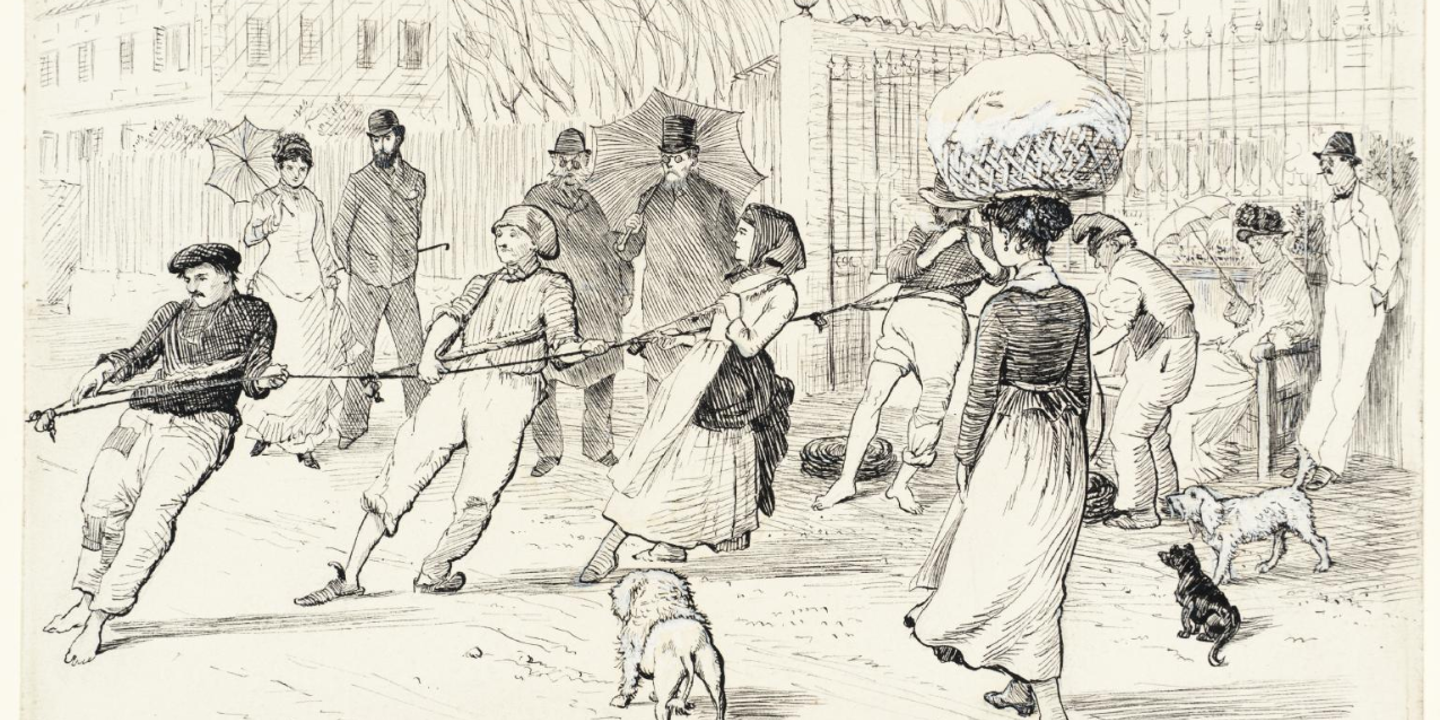
\includegraphics[width=0.5\linewidth]{Images/L6-1.png}
                \label{fig:L6-1}
            \end{figure}

            The metaphor of a tug of war conveys that economic exchanges are not one-sided acts of benevolence but rather competitive, dynamic interactions. Each party pulls in a direction dictated by self-interest, and it is in the balance of these forces that mutually beneficial outcomes emerge.

    \subsection[Of the Division of Labour]{Book I, Chapter 1\\
                \textit{Of the Division of Labour}}

        \subsubsection{Advantages of the division of labour}

            \begin{quote}
                One man draws out the wire, another straights it, a third cuts it, a fourth points it, a fifth grinds it at the top for receiving the head…
            \end{quote}

            This illustration demonstrates how breaking down production into simple, repetitive tasks can vastly increase efficiency. It shows that specialization leads to:

            \begin{itemize}
                \item Increased worker dexterity
                \item Reduction of production time, eliminating the steps from one process to another
                \item Replacement of workers with machines
            \end{itemize}

            \begin{equation}
                \text{Division of Labour} \Rightarrow Exchange \xrightarrow{but \ in \ reality}{} Exchange \Rightarrow \text{Division of Labour}
            \end{equation}

            The cyclical relationship shown in the equation reflects that specialization enhances the scope for exchange, and as trade becomes more efficient, it further encourages deeper division of labour.

    \subsection[Back to "Of the Principle which gives occasion to the Division of Labour"]{Back to Book I, Chapter 2 \\
                \textit{Of the Principle which gives occasion to the Division of Labour}}

        \subsubsection{The origin of division of labour}

            \begin{quote}
                This division of labour, from which so many advantages are derived, is not originally the effect of any human wisdom, which foresees and intends that general opulence to which it gives occasion. It is the necessary, though very slow and gradual consequence of a certain propensity in human nature which has in view no such extensive utility; the propensity to truck, barter, and exchange one thing for another.
            \end{quote}

            Smith argues that specialization is not the product of deliberate planning. Instead, it is an emergent phenomenon—an unintended consequence of humans naturally engaging in trade and exchange to meet their needs.

        \subsubsection{Exchange in primitive society}

            \begin{quote}
                In a tribe of hunters or shepherds a particular person makes bows and arrows, for example, with more readiness and dexterity than any other. He frequently exchanges them for cattle or for venison with his companions; and he finds at last that he can in this manner get more cattle and venison, than if he himself went to the field to catch them. From a regard to his own interest, therefore, the making of bows and arrows grows to be his chief business, and he becomes a sort of armourer.

                Another excels in making the frames and covers of their little huts or moveable houses. He is accustomed to be of use in this way to his neighbours, who reward him in the same manner with cattle and with venison, till at last he finds it his interest to dedicate himself entirely to this employment, and to become a sort of house-carpenter.
            \end{quote}

            This passage offers an early example of specialization. As individuals discover and refine their innate talents, they gradually assume specialized roles. In doing so, they are rewarded by their community, setting the stage for more complex economic structures.

    \subsection[That the Division of Labour is limited by the Extent of the Market]{Book I, Chapter 3 \\
                \textit{That the Division of Labour is limited by the Extent of the Market}}

        \subsubsection{No nailers in a small village}

            \begin{quote}
                It is impossible there should be such a trade as even that of a nailer in the remote and inland parts of the Highlands of Scotland. Such a workman at the rate of a thousand nails a day, and three hundred working days in the year, will make three hundred thousand nails in the year. But in such a situation it would be impossible to dispose of one thousand, that is, of one day's work in the year.
            \end{quote}

            This example illustrates that the extent of market demand restricts the scope for specialization. In a small community, the volume of trade is too limited to support highly specialized professions, emphasizing that economic growth requires a sufficiently large market.

            \begin{figure}[h]
                \centering
                \includegraphics[width=0.75\linewidth]{Images/L6-2.png}
                \label{fig:L6-2}
            \end{figure}

    \subsection[Back to "Of the Principle which gives occasion to the Division of Labour"]{Back to Book I, Chapter 2 \\
                \textit{Of the Principle which gives occasion to the Division of Labour}}

        \subsubsection{Pursuit of one’s own interest that incidentally benefits that of others}

            \begin{quote}
                Two greyhounds, in running down the same hare, have sometimes the appearance of acting in some sort of concert. Each turns her towards his companion, or endeavours to intercept her when his companion turns her towards himself. This, however, is not the effect of any contract, but of the accidental concurrence of their passions in the same object at that particular time.
            \end{quote}

            Using the metaphor of greyhounds, Smith shows that even when individuals act independently and solely out of self-interest, their actions can coincide in a manner that appears coordinated—resulting in mutual benefit without any deliberate collaboration.

        \subsubsection{While we, the human beings}

            \begin{quote}
                We address ourselves, not to their humanity but to their \textit{self-love}, and never talk to them of our own necessities but of their advantages.
            \end{quote}

            This repetition reinforces that economic transactions are driven by self-interest. Instead of appealing to the goodwill of others, individuals structure their exchanges around what benefits both parties, even if indirectly.

        \subsubsection{Self-interest?}

            \begin{quote}
                The Wealth of Nations is a stupendous palace erected upon the granite of \textit{self-interest}.

                (George Stigler, “\textit{Smith’s Travels on the Ship of State}”, 1971)
            \end{quote}

            Within this context, the correct term is not "self-interest", but it rather is "self-love"

        \subsubsection{Egoism?}

            \begin{quote}
                Ce n’est pas de la bienveillance du boucher, du marchand de bière et du boulanger, que nous attendons notre dîner, mais bien du soin qu’ils apportent à leurs intérêts. Nous ne nous adressons pas à leur humanité, mais à leur \textit{égoïsme} ; et ce n’est jamais de nos besoins que nous leur parlons, c’est toujours de leur avantage.

                (Translated by Germain Garnier, 1802)
            \end{quote}

            \begin{remark}
                Once again, French people are making confusion: here translating "self-love" with "egoism" is incorrect, as it reduces the original meaning.
            \end{remark}

        \subsubsection{Fawning dogs}

            \begin{quote}
                When an animal wants to obtain something either of a man or of another animal, it has no other means of persuasion but to gain the favour of those whose service it requires. A puppy fawns upon its dam, and a spaniel endeavours by a thousand attractions to engage the attention of its master who is at dinner, when it wants to be fed by him.
            \end{quote}

        \subsubsection{We can’t all be friends}

            \begin{quote}
                Man sometimes uses the same arts with his brethren, and when he has no other means of engaging them to act according to his inclinations, endeavours by every servile and fawning attention to obtain their good will. He has not time, however, to do this upon every occasion. In civilized society he stands at all times in need of the cooperation and assistance of great multitudes, while his whole life is scarce sufficient to gain the friendship of a few persons.
            \end{quote}

            In large societies, deep personal bonds with everyone are impossible. Instead, individuals rely on a vast network of strangers, where market relationships replace close personal ties. This dynamic underlines the necessity of self-reliance and efficient exchange.

        \subsubsection{Human beings exchange}

            \begin{quote}
                It is not from the benevolence of the butcher, the brewer, or the baker, that we expect our dinner, but from their regard to their own interest. We address ourselves, not to their humanity but to their self-love, and never talk to them of our own necessities but of their advantages.
            \end{quote}

        \subsubsection{The beggar}

            \begin{quote}
                Nobody but a beggar chuses to depend chiefly upon the benevolence of his fellow-citizens.
            \end{quote}

\section{\textit{The Theory of Moral Sentiments} (1759)}

    \subsection{The tightrope walker}

        The analogy of the tightrope walker is used to illustrate the delicate balance between individual self-interest and the need for social approval—a balance maintained through moral sentiments.

        \subsubsection{Sympathy}

            \begin{itemize}
                \item \textbf{Immediate identification}: when I see someone happy, I put myself in his situation and I start to be happy as well. Vice versa if he’s sad.\footnote{Without being a “\textit{passion contagion}” (David Hume)} 
                \begin{itemize}
                    \item \textbf{Concordance, pleasure, approval}: if there’s concordance of sentiments, there is the approval among people
                    \item \textbf{Discordance, displeasure, disapproval}: otherwise, there is disapproval towards the other
                \end{itemize}
                \item \textbf{Theory of moral judgment} based on sentiments: this is how we judge people, by having concordance or not with them.
            \end{itemize}

            \begin{remark}
                Sympathy, for Smith, is the ability to perceive and resonate with the feelings of others. This capacity is fundamental to social cohesion, as it allows us to form moral judgments and to regulate our behaviour in ways that foster mutual understanding.
            \end{remark}

            What about what we receive from the others? We want the others to give us their sympathy, so approve us. And this is the Mandeville’s self-love. 
            
            \begin{itemize}
                \item \textbf{Problem}: when we are longer in our “comfort zone”, there will always be someone to which we cannot be friends. And if this happens, we start wondering who or what is the problem (me or the other).
                \item To figure it out, according to Smith, we start putting ourselves as we were third part among the two, in order to self-judge myself and understand if the person who does not want me has reacted in a right or wrong way. 
                \begin{itemize}
                    \item If this self-judgement leads me to believe I’m doing well, this is a way to self-convince me \(\rightarrow\) self-love (Mandeville).
                \end{itemize}
            \end{itemize}

        \subsubsection{The impartial spectator}

            \begin{quote}
                When I endeavour to examine my own conduct, when I endeavour to pass sentence upon it, and either to approve or condemn it, it is evident that, in all such cases, I divide myself, as it were, into two persons; and that I, the examiner and judge, represent a different character from that other I, the person whose conduct is examined into and judged of. The first is the spectator, whose sentiments with regard to my own conduct I endeavour to enter into, by placing myself in his situation, and by considering how it would appear to me, when seen from that particular point of view. The second is the agent, the person whom I properly call myself, and of whose conduct, under the character of a spectator, I was endeavouring to form some opinion. The first is the judge; the second the person judged of.
            \end{quote}

            We prefer the approval of this third imaginary impartial spectator instead of the disapproval of that person.

            \begin{remark}
                The impartial spectator is not the internalisation of social norms and rules. This is a conformism, and according to Smith, this self-love starts from a sort of anti-conformism through which we don’t accept the other person judgement and so we look for our own judgment. 
            \end{remark}

            The concept of the impartial spectator is central to Smith’s moral philosophy. It represents an internalized voice of objectivity—an imagined observer whose perspective helps us judge our own actions fairly. This mechanism encourages self-reflection and helps maintain social norms.

            \begin{minipage}{0.48\textwidth}
                \begin{center}
                    
\includegraphics[width=0.75\linewidth]{L6-3a.png}
                    \captionof{figure}{Self-love as the pleasure of other’s approval}
                \end{center}
            \end{minipage}
            \begin{minipage}{0.04\textwidth}
                
            \end{minipage}
            \begin{minipage}{0.48\textwidth}
                \begin{center}
                    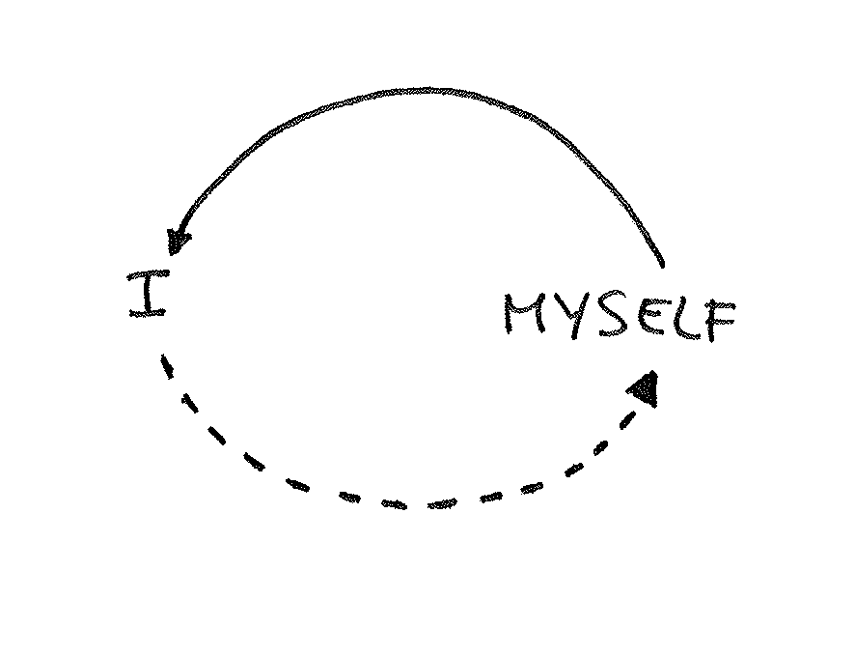
\includegraphics[width=0.75\linewidth]{L6-3b.png}
                    \captionof{figure}{Self-love as the pleasure of self-approval}
                \end{center}
            \end{minipage}

            \begin{figure}[h]
                \centering
                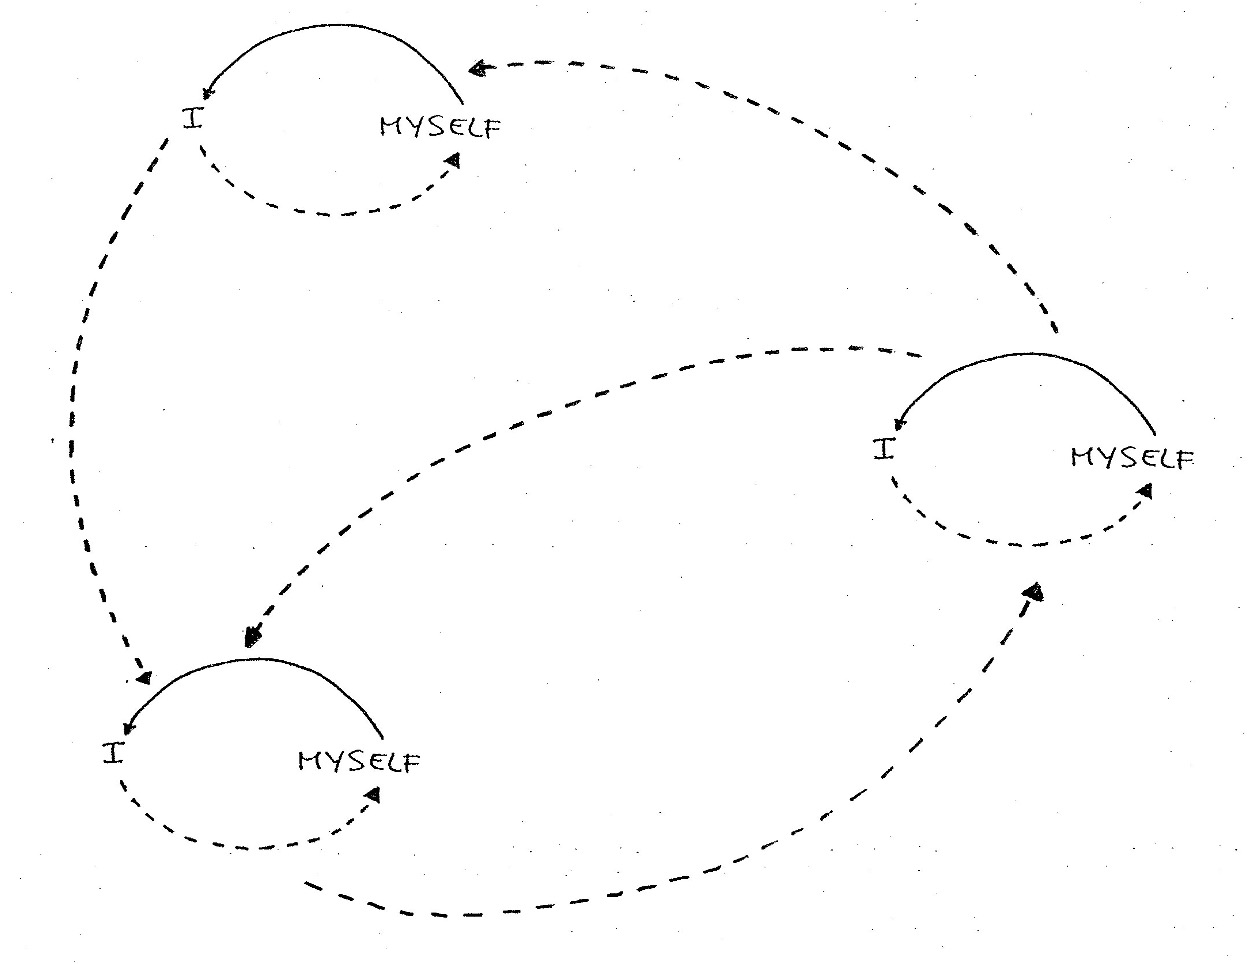
\includegraphics[width=0.32\linewidth]{L6-4.jpeg}
                \caption{Self-love as the pleasure of  deserved approval}
                \label{fig:enter-label}
            \end{figure}

\newpage
        \subsubsection{The faculty of speech}

            \begin{quote}
                Whether this propensity be one of those original principles in human nature, of which no further account can be given; or whether, as seems more probable, it be the necessary consequence of the faculties of reason and speech, it belongs not to our present subject to enquire. It is common to all men, and to be found in no other race of animals, which seem to know neither this nor any other species of contracts.
                
                Nobody ever saw a dog make a fair and deliberate exchange of one bone for another with another dog. Nobody ever saw one animal by its gestures and natural cries signify to another, this is mine, that yours; I am willing to give this for that. When an animal wants to obtain something…
            \end{quote}

             \begin{itemize}
                \item Why human beings exchange and animals do not? It is usually said that, contrary to animals, we have speech. But Smith puts it in the opposite way: speech comes out in order to exchange, because there is the propensity to exchange. We do not start to speak for other reasons but exchanging among us. 
                \item Smith says, society is a mirror; when I am in society, I know I will receive a judgement, not necessarily from the others, but also from myself that has to confront with the others.
            \end{itemize}

            This passage suggests that the faculties of reason and speech are uniquely human and have led to the development of complex social contracts and moral norms. The ability to communicate and reason underlies our capacity to negotiate, not just in economic terms, but in moral and ethical ones as well.

\section[The Pleasure of Exchange]{The pleasure of exchange: Adam Smith’s third kind of self-love}

\textbf{Question: How can we apply this third kind of self-love to exchange?}

The butcher and all other professionals find confirmation of their self-esteem in the appreciation of their work. They continue their activities only if they receive this kind of confirmation.

\begin{itemize}
    \item The person who sells apples downtown collects them in the countryside. He will continue to do so as long as buyers appreciate his efforts and validate his work by paying the agreed-upon price for the apples.
    \item The fact that buyers pay that price indicates that they appreciate the seller’s work; this recognition encourages him to keep selling apples.
\end{itemize}

\textbf{The recognition is reciprocal}: if I’m not sure the other person is truly appreciating what I do (or appreciating my goods), this will not satisfy my self-esteem, and I’ll stop providing them.

\begin{itemize}
    \item \textbf{A third element in exchange}: recognition of self-esteem.
        \begin{itemize}
            \item[\(\Rightarrow\)] Through \textbf{equivalence} (i.e., paying what the seller asks), mutual recognition is achieved.
        \end{itemize}
\end{itemize}

\begin{remark}
\begin{itemize}
    \item In a situation where there is a monopoly---where prices are imposed---exchange does not involve this mutual recognition, and therefore it lacks morality. This occurs when there is no bargaining power on both sides.
    \item Now we step outside the usual framework of \textit{non-tuism}; here, I genuinely consider the other person’s interest in the exchange. I want the other person’s satisfaction, which in turn enhances my own self-esteem. In Smith, it’s not a simple \textit{do ut des} (I give so that you might give) scenario, as exchange is often explained.
        \begin{itemize}
            \item I accept what you offer me so that I can continue to give you what you want. \textit{For instance, I don’t choose to be a professor simply for a decent salary; rather, I accept the salary because it enables me to be a professor and thus do the work I enjoy}.
            \item It is not a tug of war. The price is not merely a tool to extract maximum profit from each side before meeting in the middle. Instead, both parties look for a price that leaves them happy, given the value they each place on the good or service.
        \end{itemize}
\end{itemize}
\end{remark}

\begin{remark}
\textbf{So, are we in a society where exchange carries this moral element?} Smith says: not exactly. Mercantilists, for example, do not care about moral aspects; they seek monopolies.
    \begin{itemize}
        \item According to Smith, the situation changes in a progressive society, where workers begin to have better bargaining power with their masters. Consequently, everything improves in terms of fairness and mutual recognition.
    \end{itemize}
\end{remark}

\subsubsection{In the ‘early state’ of society}

\begin{quote}
In that early and rude state of society which precedes both the accumulation of stock and the appropriation of land, the proportion between the quantities of labour necessary for acquiring different objects seems to be the only circumstance which can afford any rule for exchanging them for one another. If among a nation of hunters, for example, it usually costs twice the labour to kill a beaver which it does to kill a deer, one beaver should naturally exchange for or be worth two deer. It is natural that what is usually the produce of two days or two hours labour, should be worth double of what is usually the produce of one day’s or one hour’s labour.

(\textit{The Wealth of Nations}, I.VI)
\end{quote}

If it takes two hours to procure a beaver and one hour to procure a deer, then one beaver = two deer. Thomas Aquinas (TA) spoke of the amount of labour as determining the value of exchange, but we also mentioned the value of exchange as discussed by Aristotle. There appears to be a tension between these views.

\begin{quote}
If the one species of labour should be more severe than the other, some allowance will naturally be made for this superior hardship; and the produce of one hour’s labour in the one way may frequently exchange for that of two hours labour in the other. Or if the one species of labour requires an uncommon degree of dexterity and ingenuity, the esteem which men have for such talents, will naturally give a value to their produce, superior to what would be due to the time employed about it. Such talents can seldom be acquired but in consequence of long application, and the superior value of their produce may frequently be no more than a reasonable compensation for the time and labour which must be spent in acquiring them.

(\textit{The Wealth of Nations}, I.VI)
\end{quote}

The key point is that certain qualitative factors must be accounted for in the “quantity of labour,” and we must agree on their value. Thus, hardship and ingenuity must also be evaluated.

\subsubsection{Hardship and ingenuity}

\begin{quote}
It is often difficult to ascertain the proportion between two different quantities of labour. The time spent in two different sorts of work will not always alone determine this proportion. The different degrees of hardship endured, and of ingenuity exercised, must likewise be taken into account. There may be more labour in an hour’s hard work than in two hours easy business; or in an hour’s application to a trade which it cost ten years labour to learn, than in a month’s industry at an ordinary and obvious employment.

(\textit{The Wealth of Nations}, I.V)
\end{quote}

\begin{remark}
There may be more labour in one hour of hard work than in two hours of easier work. Thus, we cannot rely solely on a static, simplistic proportion from the “early state” model.
\end{remark}

\subsubsection{In the ‘advanced state’ of society}

\begin{quote}
In the advanced state of society, allowances of this kind, for superior hardship and superior skill, are commonly made in the wages of labour; and something of the same kind must probably have taken place in its earliest and rudest period.

(\textit{The Wealth of Nations}, I.VI)
\end{quote}

\subsection{A contraposition of theories of value}

\subsubsection{Aquinas’ theory of value}

\begin{quote}
If a farmer gave a bushel of wheat for a sandal, he would have an excess of labor in his product (“superabundantiam laboris in opere”) and would have also an excess of presents (“superabundantiam doni”) because he would be giving more than he would receive. But when all have what is theirs, they are in this way equal and do business with one another because the equality previously mentioned is possible for them.

(\textit{Summa Theologiae})
\end{quote}

\subsubsection{Smith’s theory of value}

\begin{quote}
Exchanged goods “contain the value of a certain quantity of labour which we exchange for what is supposed at the time to contain the value of an equal quantity.”

(\textit{The Wealth of Nations}, I.V)
\end{quote}

\subsubsection{Back to “Hardship and ingenuity”}

\begin{quote}
But it is not easy to find any accurate measure either of hardship or ingenuity. In exchanging indeed the different productions of different sorts of labour for one another, some allowance is commonly made for both. It is adjusted, however, not by any accurate measure, but by the higgling and bargaining of the market, according to that sort of rough equality which, though not exact, is sufficient for carrying on the business of common life.

(\textit{The Wealth of Nations}, I.V)
\end{quote}

\begin{remark}
I recognize your hardship and you recognize my ingenuity in the process of exchanging. Otherwise, these considerations would not come to light. It happens only through negotiation.
\end{remark}

\section*{Additional Context and Observations}

\begin{remark}
Both \textit{The Wealth of Nations} and \textit{The Theory of Moral Sentiments} are best understood in the context of the Enlightenment. Smith’s work not only laid the groundwork for modern economics but also offered profound insights into human behavior, ethics, and the emergence of social institutions.
\end{remark}

\begin{remark}
The juxtaposition of economic self-interest and moral sentiment is central to Smith’s philosophy. While self-interest propels market transactions, our capacity for sympathy and our internal judgment (the impartial spectator) help maintain social order and ethical behavior.
\end{remark}

\begin{remark}
The recurring theme of self-interest---whether expressed as the invisible hand in market transactions or as the pursuit of self-approval in moral judgment---suggests that human behavior, though seemingly divided between economic and moral spheres, is underpinned by a consistent set of motivations.
\end{remark}

\begin{remark}
Smith’s observations about the division of labour and the size of the market show that economic specialization is both enabled and constrained by social structures. Similarly, the development of moral sentiments is linked to the unique human capacity for language and reflection.
\end{remark}


    \chapter[Private property and communism]{Karl Marx \\[0.6cm] \textit{Private property and communism}}

    \chapter[Perfect competition and paradox of uncertainty]{Franck Knight\\[0.6cm] \textit{Perfect competition and the paradox of uncertainty}}

\part{Readings for the First Part}

    \setcounter{chapter}{0}
    \chapter[\textit{Nichomachean Ethics}, Chapter III-V]{Aristotle \\ \textit{Nichomachean Ethics}, Chapter III-V}

    \setcounter{chapter}{2}
    \chapter[\textit{Leviathan}, Chapter I]{Thomas Hobbes \\ \textit{Leviathan}, Chapter I}

    \chapter[\textit{The Fable of the Bees}, Remark B]{Bernard de Mandeville \\ \textit{The Fable of the Bees}, Remark B}

    \setcounter{chapter}{5}
    \chapter[\textit{The Wealth of Nations}, Chapter II]{Adam Smith \\ \textit{The Wealth of Nations}, Chapter II}

    \setcounter{chapter}{5}
    \chapter[\textit{The Wealth of Nations}, Chapter VII]{Adam Smith \\ \textit{The Wealth of Nations}, Chapter VII}

    
    

\end{document}
